% !TEX root = ../Thesis.tex
\chapter{Evaluation}

Now it is time to see how PINCH stacks up against its non incremental counterpart Generalized Dijkstra by comparing the two algorithms in a variety of domains.

\section{Summary of Methods}
For our implementation we have used the \href{http://www.fast-downward.org/}{Fast Downward Planner}. The search component of the planner is written in c++. For our evaluation we compare (improved) PINCH and GD. Both algorithms use a bucket based priority queue.\\

For the comparison we will use weighted A* with a weight of 2. The algorithms are compared on a big collection of domains (Satisficing Track of IPC 1998-2018) with in total 2542 instances. The instances induce state spaces with action costs $>$ 0. We track a number of factors such as coverage, search time and different types of errors.\\

The experiments were done at the \href{https://scicore.unibas.ch/}{center for scientific computing (sciCORE)} in Basel. 

\newpage
\section{Evaluation}
\subsection{General Overview}
I want to start the evaluation by giving a basic picture of what the results are like.\\
\begin{table}[h]
\begin{longtable}[c]{| c | c | c |}
     \hline
     \multicolumn{3}{| c |}{Results}\\
     \hline
     Property & GD & PINCH\\
     \hline
     \endfirsthead
     \hline
     \endfoot
     Number of Runs & 2542 & 2542\\
     Coverage & 1663 & 1630\\
     Search out of Memory & 138 & 229\\
     Search out of Time & 696 & 638\\
     Search Time & 1.08 & 1.84\\
     \hline
\end{longtable}
\caption*{Table 4.1: Summary of the Results, Search Time is the mean Search Time in seconds over all Runs}
\end{table}\\
Let us discuss the Results that we can see in Table 4.1. The coverage, meaning the number of instances for which a plan was found, is comparable between the 2 algorithms. GD covers a slightly larger amount, which will make sense as we continue to explore the evaluation. Search out of Memory and Search out of Time tells us how many runs were interrupted either due to memory or time constraints, the planning time was restricted to 30 minutes and the memory to 3584Mib. PINCH runs out of memory more often than GD, this is likely due to the priority queue storing both variables and actions in PINCH, whereas GD only stores variables.\\

Perhaps the most interesting property is the Search Time. GD, on average, finds plans about 1.7 times more quickly than PINCH.
\subsection{Search Time}
We have just seen that GD outperforms PINCH on average by a significant margin. Figure 4.1 shows us how GD and PINCH compare in terms of search time. The further away an entry is from the diagonal line, the bigger the disparity for that entry between the two algorithms. Here we can see that, while GD outperforms PINCH on average, PINCH clearly has plenty of instances in its favour. To be exact, PINCH outperforms GD on 449 of the 2542 instances. Assuming that PINCH and GD roughly cover the same instances, that would be 449 of the $\sim$1600 covered instances, meaning PINCH outperforms GD on circa one fourth of the covered instances.

\begin{figure}
    \centering
    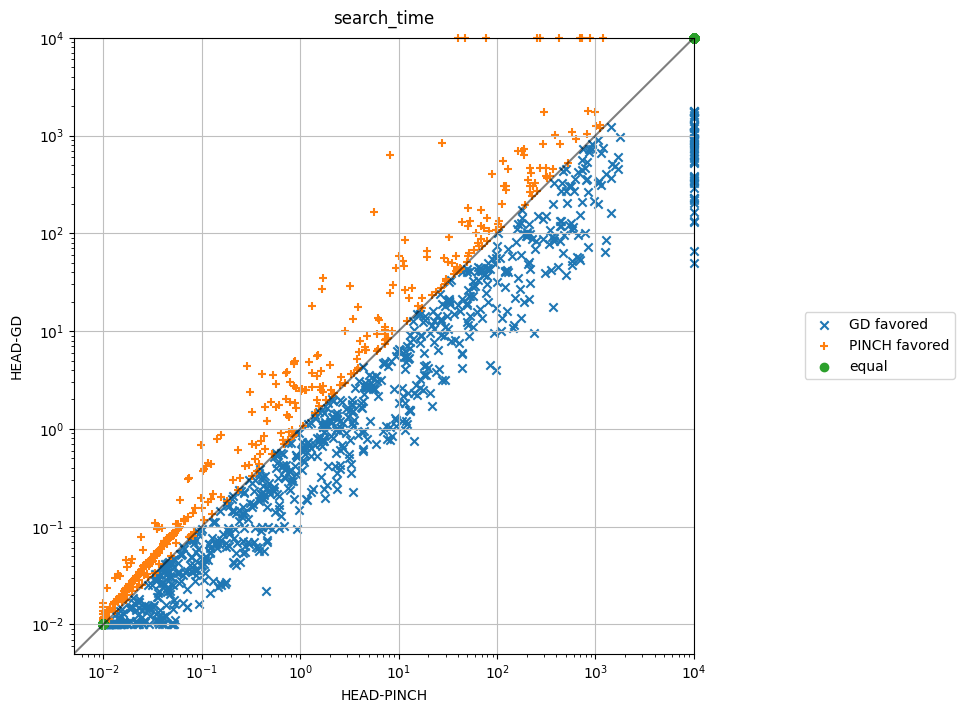
\includegraphics[width=1\columnwidth]{plotSearchimpr.png}
    \caption{Search Time comparison Plot}
    \label{fig:my_label}
\end{figure}
\newpage
I now want to explore the reasons for the inconsistent performance of PINCH. In order to do this I have selected several domains from the set of domains in which PINCH either performs exceptionally well, about the same as GD or significantly worse than GD (Table 4.2). The PINCH and GD favored domains were chosen based on the number of instances in the domains and the degree to which either algorithm outperforms the other one. The PINCH and GD favored domains are the 4 \textit{best} domains for either algorithm when comparing mean search time. The domains for the Equal grouping were chosen based on the number of instances in the domains and the similarity in performance between PINCH and GD. The domains in the Equal grouping are the 3 most similar domains between PINCH and GD when comparing mean search time.

\begin{table}[h]
\begin{longtable}[c]{| c | c | c |}
     \hline
     \multicolumn{3}{| c |}{Domain Groups}\\
     \hline
     \textcolor{green}{{\small PINCH favored}} & \textcolor{blue}{{\small Equal}} & \textcolor{red}{{\small GD favored}}\\
     \hline
     \endfirsthead
     \hline
     \endfoot
     {\small satellite (SAT)}& {\small miconic-fulladl (MIC)}& {\small freecell (FRE)}\\
     {\small logistics98 (LOG) }& {\small caldera-sat18-adl (CAL)}& {\small pipesworld-notankage (PIP)}\\
     {\small woodworking-sat11-strips (WOO)}& {\small schedule (SCH)}& {\small spider-sat18-strips (SPI)}\\
     {\small maintenance-sat14-adl (MAI)}&  & {\small agricola-sat18-strips (AGR)}\\
     \hline
\end{longtable}
\caption*{Table 4.2: grouping of domains according to search time performance}
\end{table}

\newpage
Going forward we will often use the abbreviations that you can see in parenthesis in Table 4.2 to refer to the domains. We will also use the colors from Table 4.2 (green/blue/red) to show which domain is part of which group. If we plot only the instances from the domains from Table 4.2 the plot looks as follows:\\
\begin{figure}
    \centering
    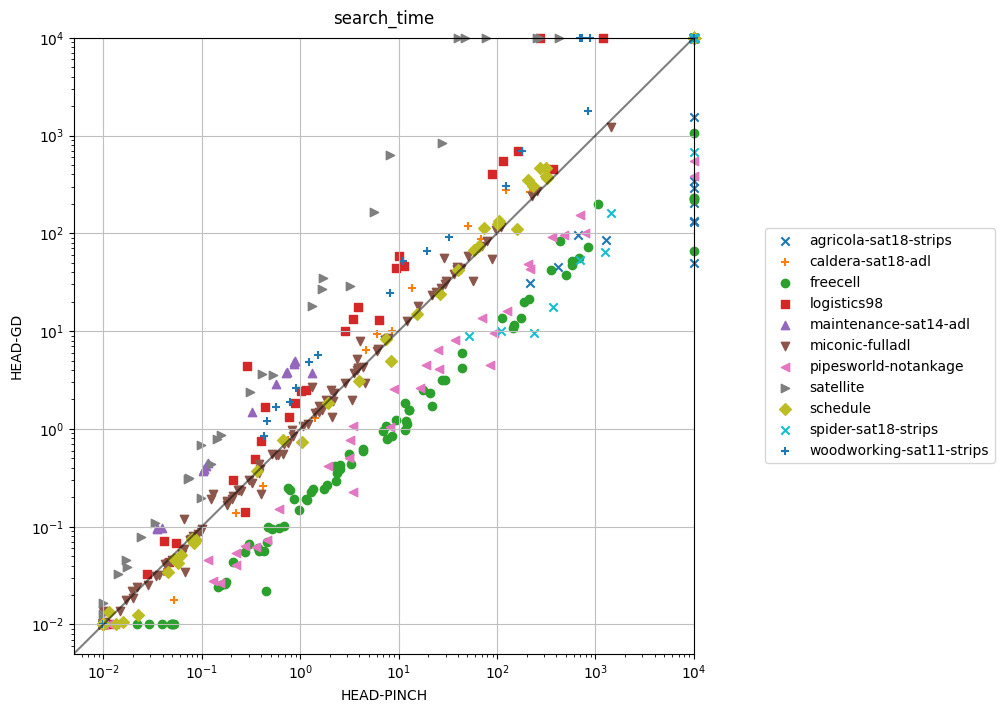
\includegraphics[width=1\columnwidth]{plotSearchDomainGroups.png}
    \caption{Search Time comparison Plot for the instances from the domains from Table 4.2}
    \label{fig:my_label}
\end{figure}\\
Interesting to note is that the instances in the PINCH favored and GD favored groupings consistently outperform and have a tendency to outperform more strongly with increasing size. The instances from the Equal group tend to favor GD on small instance sizes and slowly start to favor PINCH with increasing size. \\

Now that we have selected our domains, we will analyze these domains for information that might explain the performance of PINCH.

\subsection{The Incremental Benefit}
The main difference between GD and PINCH are the incremental calculations that PINCH uses. In order for us to quantify how big the incremental benefit is that PINCH can derive from a given instance, we have to come up with factors that are related to the incremental benefit.\\

\subsubsection{Introducing the Factors}
I want to explain the factors that I use to quantify the incremental benefit by demonstrating them on our example from chapter 3.2. Remember that the final result of the Example from chapter 3.2 looks as follows:

% !TEX root = ../Thesis.tex


\date{April 29, 2020}

%% TODO: This needs to be shortened a bit. In 2013, this lecture was
%% 5-10 minutes too long (I managed it in one session but ran over)
%% without being too slow or too fast. We can probably get rid of the
%% 15-puzzle stuff, moving it to the exercises to make some time. And
%% a not-RPG-centric description of h^max/h^add/h^FF could probably
%% also be done faster than the current RPG-centric one.

\usetikzlibrary{shapes}

\tikzstyle{relaxed planning graph}=[draw,inner sep=0pt,font=\small]
\tikzstyle{rpg square}=[relaxed planning graph,minimum size=0.52cm,rectangle]
\tikzstyle{rpg circle}=[relaxed planning graph,minimum size=0.52cm,circle]

\tikzstyle{prop}=        [rpg circle,fill=yellow]
\tikzstyle{notthere}=    [color=gray!15,fill=gray!5]
\tikzstyle{operator}=    [rpg square,fill=blue!40]
\tikzstyle{selected}=[fill=cyan]

\tikzstyle{goalachieved}=[fill=red!50]
\tikzstyle{solved} = [fill=green!30]
\tikzstyle{lockedin} = [fill=blue!30]
\tikzstyle{assignedprop}=[rpg circle,fill=orange!40]
\tikzstyle{assignedoperator}=[rpg square,fill=orange!40]

\tikzstyle{idle}=[thin]
\tikzstyle{nonidle}=[thin]
\tikzstyle{arc selected}=[color=cyan,very thick]

\newcommand{\markplusone}[1]{\path (#1) +(-0.04cm,0.28cm) node {\tiny $+1$};}
\newcommand{\markopnode}[3][0.35cm]{\path (#2) +(0cm,#1) node {\tiny
    \ensuremath{#3}};}
\newcommand{\markopnodeff}[3][0.30cm]{\path (#2) +(0cm,#1) node {\tiny
    \ensuremath{#3}};}
\newcommand{\markopcost}[2]{\path (#1) +(0.45cm,0.15cm) node {\tiny $+#2$};}

\newcommand{\pre}{\ensuremath{\textit{pre}}}
\newcommand{\add}{\ensuremath{\textit{add}}}
\newcommand{\del}{\ensuremath{\textit{del}}}
\newcommand{\relaxation}[1]{\ensuremath{#1^+}}
\newcommand{\hplus}{\ensuremath{h^+}}
\newcommand{\hmax}{\ensuremath{h^{\textup{max}}}}
\newcommand{\hadd}{\ensuremath{h^{\textup{add}}}}
\newcommand{\hff}{\ensuremath{h^{\textup{FF}}}}



  %% TODO: Got rid of centering to avoid the graph jumping.
  %% Should find a better solution for this.
  %% \begin{center}
\begin{center}
\begin{minipage}[t]{.7\linewidth}
\vspace{-10pt}
\centering
\begin{frame}{}
    \begin{tikzpicture}
      \pgfsetxvec{\pgfpoint{2.77cm}{0.0cm}}
      \pgfsetyvec{\pgfpoint{0.0cm}{0.87cm}}
      %% variable layer 0
      \only<1->{
        \node[prop, lockedin] at (0.0,7.0) (a0) {0};
        \node[prop, notthere] at (0.0,6.0) (b0) {$b^0$};
        \node[prop, solved] at (0.0,5.0) (c0) {0};
        \node[prop,notthere] at (0.0,4.0) (d0) {$d^0$};
        \node[prop,notthere] at (0.0,3.0) (e0) {$e^0$};
        \node[prop,notthere] at (0.0,2.0) (f0) {$f^0$};
        \node[prop,notthere] at (0.0,1.0) (g0) {$g^0$};
        \node[prop,notthere] at (0.0,0.0) (h0) {$h^0$};
      }
      %% action layer 1
      \only<2->{
        %% action a_1
        \node[operator, lockedin] at (0.5,6.5) (o1-1) {1};
        \markopcost{o1-1}{1};
        \draw[->,nonidle] (a0)--(o1-1);
        \node[operator, solved] at (0.5,5.5) (o2-1) {1};
        \markopcost{o2-1}{1};
        \draw[->,nonidle] (a0)--(o2-1);
        \draw[->,nonidle] (c0)--(o2-1);
      }
      %% variable layer 1
      \only<3->{
        \node[prop, lockedin] at (1.0,7.0) (a1) {0};
        \node[prop, solved] at (1.0,6.0) (b1) {2};
        \node[prop, solved] at (1.0,5.0) (c1) {0};
        \node[prop, solved] at (1.0,4.0) (d1) {2};
        \node[prop,notthere] at (1.0,3.0) (e1) {$e^1$};
        \node[prop, notthere] at (1.0,2.0) (f1) {$f^1$};
        \node[prop,notthere] at (1.0,1.0) (g1) {$g^1$};
        \node[prop,notthere] at (1.0,0.0) (h1) {$h^1$};
        %% idle arcs
        \draw[->,idle] (a0)--(a1);
        \draw[->,idle,notthere] (b0)--(b1);
        \draw[->,idle] (c0)--(c1);
        \draw[->,idle,notthere] (d0)--(d1);
        \draw[->,idle,notthere] (e0)--(e1);
        \draw[->,idle,notthere] (f0)--(f1);
        \draw[->,idle,notthere] (g0)--(g1);
        \draw[->,idle,notthere] (h0)--(h1);
        %% effect arcs
        \draw[->,nonidle] (o1-1)--(b1);
        \draw[->,nonidle] (o1-1)--(c1);
        \draw[->,nonidle] (o2-1)--(d1);
      }
      %% action layer 2
      \only<4->{
        %% action a_1
        \node[operator, lockedin] at (1.5,6.5) (o1-2) {1};
        \markopcost{o1-2}{1};
        \draw[->,nonidle] (a1)--(o1-2);
        %% action a_2
        \node[operator, solved] at (1.5,5.5) (o2-2) {1};
        \markopcost{o2-2}{1};
        \draw[->,nonidle] (a1)--(o2-2);
        \draw[->,nonidle] (c1)--(o2-2);
        %% action a_3
        \node[operator, solved] at (1.5,4.5) (o3-2) {3};
        \markopcost{o3-2}{1};
        \draw[->,nonidle] (b1)--(o3-2);
        \draw[->,nonidle] (c1)--(o3-2);
        %% action a_4
        \node[operator, solved] at (1.5,3.5) (o4-2) {3};
        \markopcost{o4-2}{1};
        \draw[->,nonidle] (b1)--(o4-2);
         %% action a_5
        \node[operator, solved] at (1.5,2.5) (o5-2) {3};
        \markopcost{o5-2}{1};
        \draw[->,nonidle] (d1)--(o5-2);
        %% action a_6
        \node[operator, solved] at (1.5,1.5) (o6-2) {3};
        \markopcost{o6-2}{1};
        \draw[->,nonidle] (d1)--(o6-2);
      }
      %% variable layer 2
      \only<5->{
        \node[prop, lockedin] at (2.0,7.0) (a2) {0};
        \node[prop, solved] at (2.0,6.0) (b2) {2};
        \node[prop, solved] at (2.0,5.0) (c2) {0};
        \node[prop, solved] at (2.0,4.0) (d2) {2};
        \node[prop, solved] at (2.0,3.0) (e2) {4};
        \node[prop, solved] at (2.0,2.0) (f2) {4};
        \node[prop, solved] at (2.0,1.0) (g2) {4};
        \node[prop,notthere] at (2.0,0.0) (h2) {$h^2$};
        %% effect arcs
        \draw[->,nonidle] (o1-2)--(b2);
        \draw[->,nonidle] (o1-2)--(c2);
        \draw[->,nonidle] (o2-2)--(d2);
        \draw[->,nonidle] (o3-2)--(e2);
        \draw[->,nonidle] (o4-2)--(f2);
        \draw[->,nonidle] (o5-2)--(e2);
        \draw[->,nonidle] (o5-2)--(f2);
        \draw[->,nonidle] (o6-2)--(g2);
        %% idle arcs
        \draw[->,idle] (a1)--(a2);
        \draw[->,idle] (b1)--(b2);
        \draw[->,idle] (c1)--(c2);
        \draw[->,idle] (d1)--(d2);
        \draw[->,idle,notthere] (e1)--(e2);
        \draw[->,idle, notthere] (f1)--(f2);
        \draw[->,idle,notthere] (g1)--(g2);
        \draw[->,idle,notthere] (h1)--(h2);
      }
      %% action layer 3
      \only<6->{
        %% action a_1
%        \node[operator, solved] at (2.5,6.5) (o1-3) {3};
%        \draw[->,nonidle] (a2)--(o1-3);
        %% action a_2
%        \node[operator, solved] at (2.5,5.5) (o2-3) {1};
%        \draw[->,nonidle] (a2)--(o2-3);
%        \draw[->,nonidle] (c2)--(o2-3);
        %% action a_3
%        \node[operator, solved] at (2.5,4.5) (o3-3) {7};
%        \draw[->,nonidle] (b2)--(o3-3);
%        \draw[->,nonidle] (c2)--(o3-3);
        %% action a_4
%        \node[operator, solved] at (2.5,3.5) (o4-3) {7};
%        \draw[->,nonidle] (b2)--(o4-3);
        %% action a_5
%        \node[operator, solved] at (2.5,2.5) (o5-3) {3};
%        \draw[->,nonidle] (d2)--(o5-3);
        %% action a_6
%        \node[operator, solved] at (2.5,1.5) (o6-3) {3};
%        \draw[->,nonidle] (d2)--(o6-3);
      }
      %% variable layer 3
      \only<7->{
        \node[prop, notthere] at (3.0,7.0) (a3) {$a^3$};
        \node[prop, notthere] at (3.0,6.0) (b3) {$b^3$};
        \node[prop, notthere] at (3.0,5.0) (c3) {$c^3$};
        \node[prop, notthere] at (3.0,4.0) (d3) {$d^3$};
        \node[prop, notthere] at (3.0,3.0) (e3) {$e^3$};
        \node[prop, notthere] at (3.0,2.0) (f3) {$f^3$};
        \node[prop, notthere] at (3.0,1.0) (g3) {$g^3$};
        \node[prop,notthere] at (3.0,0.0) (h3) {$h^3$};
        %% effect arcs
%        \draw[->,nonidle] (o1-3)--(b3);
%        \draw[->,nonidle] (o1-3)--(c3);
%        \draw[->,nonidle] (o2-3)--(d3);
%        \draw[->,nonidle] (o3-3)--(e3);
%        \draw[->,nonidle] (o4-3)--(f3);
%        \draw[->,nonidle] (o5-3)--(e3);
%        \draw[->,nonidle] (o5-3)--(f3);
%        \draw[->,nonidle] (o6-3)--(g3);
        %% idle arcs
        \draw[->,idle,notthere] (a2)--(a3);
        \draw[->,idle,notthere] (b2)--(b3);
        \draw[->,idle,notthere] (c2)--(c3);
        \draw[->,idle,notthere] (d2)--(d3);
        \draw[->,idle,notthere] (e2)--(e3);
        \draw[->,idle,notthere] (f2)--(f3);
        \draw[->,idle,notthere] (g2)--(g3);
        \draw[->,idle,notthere] (h2)--(h3);
      }
      \only<beamer:8|handout:0>{
        \node[prop,solved] at (2.0,5.0) (c3) {0};
        \node[prop,solved] at (2.0,4.0) (d3) {2};
        \node[prop,solved] at (2.0,3.0) (e3) {4};
        \node[prop,solved] at (2.0,2.0) (f3) {4};
        \node[prop,solved] at (2.0,1.0) (g3) {4};
      }
      \only<9->{
        \node[operator,goalachieved] at (2.5,3.0) (G) {14};
        \draw[->,nonidle] (c3)--(G);
        \draw[->,nonidle] (d3)--(G);
        \draw[->,nonidle] (e3)--(G);
        \draw[->,nonidle] (f3)--(G);
        \draw[->,nonidle] (g3)--(G);
      }
    \end{tikzpicture}
    $\hadd(s) = 14/2 = 7$
  %% \end{center}
   %% \end{center}
\end{frame}
\end{minipage}%
\begin{minipage}[t]{.4\linewidth}
\vspace{-35pt}
\centering
\begin{longtable}[c]{| c | c | c|}
     \hline
     \multicolumn{3}{| c |}{new state s}\\
     \hline
     $q$ & $x_q$ & $rhs_q$\\
     \hline
     \endfirsthead
     \hline
     \endfoot
     $a$ & 0 & 0\\
     $b$ & 2 & 2\\
     $c$ & 0 & 0\\
     $d$ & 2 & 2\\
     $e$ & 4 & 4\\
     $f$ & 4 & 4\\
     $g$ & 4 & 4\\
     $a_1$ & 1 & 1\\
     $a_2$ & 1 & 1\\
     $a_3$ & 3 & 3\\
     $a_4$ & 3 & 3\\
     $a_5$ & 3 & 3\\
     $a_6$ & 3 & 3\\
     \hline
\end{longtable}
\end{minipage}
\end{center}


The blue nodes tell us which $q$ did not have to be recalculated and were taken over from $s'$. In this example $s$ and $s'$ were set as follows:
\begin{multicols}{2}
\begin{itemize}
\setlength\itemsep{0em}
\item $s' = I = \{a,b\}$
\item $s = \{a,c\}$
\end{itemize}
\end{multicols}
Now lets consider a new example with the same state space from chapter 3.2 but with:
\begin{center}
\begin{multicols}{2}
\begin{itemize}
\setlength\itemsep{0em}
\item $s' = \{a,b,c,d\}$
\item $s = \{a,b,c,d,e\}$
\end{itemize}
\end{multicols}
\end{center}
The final result for $s'$ in this instance looks as follows:
% !TEX root = ../Thesis.tex


\subtitle{}
\date{April 29, 2020}

%% TODO: This needs to be shortened a bit. In 2013, this lecture was
%% 5-10 minutes too long (I managed it in one session but ran over)
%% without being too slow or too fast. We can probably get rid of the
%% 15-puzzle stuff, moving it to the exercises to make some time. And
%% a not-RPG-centric description of h^max/h^add/h^FF could probably
%% also be done faster than the current RPG-centric one.

\usetikzlibrary{shapes}

\tikzstyle{relaxed planning graph}=[draw,inner sep=0pt,font=\small]
\tikzstyle{rpg square}=[relaxed planning graph,minimum size=0.52cm,rectangle]
\tikzstyle{rpg circle}=[relaxed planning graph,minimum size=0.52cm,circle]

\tikzstyle{prop}=        [rpg circle,fill=yellow]
\tikzstyle{notthere}=    [color=gray!15,fill=gray!5]
\tikzstyle{operator}=    [rpg square,fill=blue!40]
\tikzstyle{selected}=[fill=cyan]

\tikzstyle{goalachieved}=[fill=red!50]
\tikzstyle{solved} = [fill=green!30]
\tikzstyle{lockedin} = [fill=blue!30]
\tikzstyle{assignedprop}=[rpg circle,fill=orange!40]
\tikzstyle{assignedoperator}=[rpg square,fill=orange!40]

\tikzstyle{idle}=[thin]
\tikzstyle{nonidle}=[thin]
\tikzstyle{arc selected}=[color=cyan,very thick]

\newcommand{\markplusone}[1]{\path (#1) +(-0.04cm,0.28cm) node {\tiny $+1$};}
\newcommand{\markopnode}[3][0.35cm]{\path (#2) +(0cm,#1) node {\tiny
    \ensuremath{#3}};}
\newcommand{\markopnodeff}[3][0.30cm]{\path (#2) +(0cm,#1) node {\tiny
    \ensuremath{#3}};}
\newcommand{\markopcost}[2]{\path (#1) +(0.45cm,0.15cm) node {\tiny $+#2$};}

\newcommand{\pre}{\ensuremath{\textit{pre}}}
\newcommand{\add}{\ensuremath{\textit{add}}}
\newcommand{\del}{\ensuremath{\textit{del}}}
\newcommand{\relaxation}[1]{\ensuremath{#1^+}}
\newcommand{\hplus}{\ensuremath{h^+}}
\newcommand{\hmax}{\ensuremath{h^{\textup{max}}}}
\newcommand{\hadd}{\ensuremath{h^{\textup{add}}}}
\newcommand{\hff}{\ensuremath{h^{\textup{FF}}}}



  %% TODO: Got rid of centering to avoid the graph jumping.
  %% Should find a better solution for this.
  %% \begin{center}
\begin{center}
\begin{minipage}[t]{.7\linewidth}
\vspace{-22pt}
\centering
\begin{frame}{}
    \begin{tikzpicture}
      \pgfsetxvec{\pgfpoint{2.77cm}{0.0cm}}
      \pgfsetyvec{\pgfpoint{0.0cm}{0.87cm}}
      %% variable layer 0
      \only<1->{
        \node[prop, solved] at (0.0,7.0) (a0) {0};
        \node[prop, solved] at (0.0,6.0) (b0) {0};
        \node[prop, solved] at (0.0,5.0) (c0) {0};
        \node[prop,solved] at (0.0,4.0) (d0) {0};
        \node[prop,notthere] at (0.0,3.0) (e0) {$e^0$};
        \node[prop,notthere] at (0.0,2.0) (f0) {$f^0$};
        \node[prop,notthere] at (0.0,1.0) (g0) {$g^0$};
        \node[prop,notthere] at (0.0,0.0) (h0) {$h^0$};
      }
      %% action layer 1
      \only<2->{
        %% action a_1
        \node[operator, solved] at (0.5,6.5) (o1-1) {1};
        \draw[->,nonidle] (a0)--(o1-1);
        \markopcost{o1-1}{1};
        %% action a_2
        \node[operator, solved] at (0.5,5.5) (o2-1) {1};
        \markopcost{o2-1}{1};
        \draw[->,nonidle] (a0)--(o2-1);
        \draw[->,nonidle] (c0)--(o2-1);
        %% action a_3
        \node[operator, solved] at (0.5,4.5) (o3-1) {1};
        \markopcost{o3-1}{1};
        \draw[->,nonidle] (b0)--(o3-1);
        \draw[->,nonidle] (c0)--(o3-1);
        %% action a_4
        \node[operator, solved] at (0.5,3.5) (o4-1) {1};
        \markopcost{o4-1}{1};
        \draw[->,nonidle] (b0)--(o4-1);
         %% action a_5
        \node[operator, solved] at (0.5,2.5) (o5-1) {1};
        \markopcost{o5-1}{1};
        \draw[->,nonidle] (d0)--(o5-1);
        %% action a_6
        \node[operator, solved] at (0.5,1.5) (o6-1) {1};
        \markopcost{o6-1}{1};
        \draw[->,nonidle] (d0)--(o6-1);
      }
      %% variable layer 1
      \only<3->{
        \node[prop, solved] at (1.0,7.0) (a1) {0};
        \node[prop, solved] at (1.0,6.0) (b1) {0};
        \node[prop, solved] at (1.0,5.0) (c1) {0};
        \node[prop, solved] at (1.0,4.0) (d1) {0};
        \node[prop,solved] at (1.0,3.0) (e1) {2};
        \node[prop, solved] at (1.0,2.0) (f1) {2};
        \node[prop,solved] at (1.0,1.0) (g1) {2};
        \node[prop,notthere] at (1.0,0.0) (h1) {$h^1$};
        %% idle arcs
        \draw[->,idle] (a0)--(a1);
        \draw[->,idle] (b0)--(b1);
        \draw[->,idle] (c0)--(c1);
        \draw[->,idle] (d0)--(d1);
        \draw[->,idle,notthere] (e0)--(e1);
        \draw[->,idle,notthere] (f0)--(f1);
        \draw[->,idle,notthere] (g0)--(g1);
        \draw[->,idle,notthere] (h0)--(h1);
        %% effect arcs
        \draw[->,nonidle] (o1-1)--(b1);
        \draw[->,nonidle] (o1-1)--(c1);
        \draw[->,nonidle] (o2-1)--(d1);
        \draw[->,nonidle] (o3-1)--(e1);
        \draw[->,nonidle] (o4-1)--(f1);
        \draw[->,nonidle] (o5-1)--(e1);
        \draw[->,nonidle] (o5-1)--(f1);
        \draw[->,nonidle] (o6-1)--(g1);
      }
      %% action layer 2
      \only<4->{
        %% action a_1
%        \node[operator, lockedin] at (1.5,6.5) (o1-2) {3};
%        \markopcost{o1-2}{3};
%        \draw[->,nonidle] (a1)--(o1-2);
        %% action a_2
%        \node[operator, solved] at (1.5,5.5) (o2-2) {7};
%        \draw[->,nonidle] (a1)--(o2-2);
%        \draw[->,nonidle] (c1)--(o2-2);
        %% action a_3
%        \node[operator, solved] at (1.5,4.5) (o3-2) {7};
%        \markopcost{o3-2}{1};
%        \draw[->,nonidle] (b1)--(o3-2);
%        \draw[->,nonidle] (c1)--(o3-2);
        %% action a_4
%        \node[operator, solved] at (1.5,3.5) (o4-2) {1};
%        \markopcost{o4-2}{1};
%        \draw[->,nonidle] (b1)--(o4-2);
         %% action a_5
%        \node[operator, solved] at (1.5,2.5) (o5-2) {3};
%        \markopcost{o5-2}{1};
%        \draw[->,nonidle] (d1)--(o5-2);
        %% action a_6
%        \node[operator, solved] at (1.5,1.5) (o6-2) {3};
%        \markopcost{o6-2}{1};
 %       \draw[->,nonidle] (d1)--(o6-2);
      }
      %% variable layer 2
      \only<5->{
        \node[prop, notthere] at (2.0,7.0) (a2) {$a^2$};
        \node[prop, notthere] at (2.0,6.0) (b2) {$b^2$};
        \node[prop, notthere] at (2.0,5.0) (c2) {$c^2$};
        \node[prop, notthere] at (2.0,4.0) (d2) {$d^2$};
        \node[prop, notthere] at (2.0,3.0) (e2) {$e^2$};
        \node[prop, notthere] at (2.0,2.0) (f2) {$f^2$};
        \node[prop, notthere] at (2.0,1.0) (g2) {$g^2$};
        \node[prop,notthere] at (2.0,0.0) (h2) {$h^2$};
        %% effect arcs
 %       \draw[->,nonidle] (o1-2)--(b2);
 %       \draw[->,nonidle] (o1-2)--(c2);
 %       \draw[->,nonidle] (o2-2)--(d2);
 %       \draw[->,nonidle] (o3-2)--(e2);
 %       \draw[->,nonidle] (o4-2)--(f2);
 %       \draw[->,nonidle] (o5-2)--(e2);
 %       \draw[->,nonidle] (o5-2)--(f2);
 %       \draw[->,nonidle] (o6-2)--(g2);
        %% idle arcs
        \draw[->,idle, notthere] (a1)--(a2);
        \draw[->,idle, notthere] (b1)--(b2);
        \draw[->,idle,notthere] (c1)--(c2);
        \draw[->,idle,notthere] (d1)--(d2);
        \draw[->,idle,notthere] (e1)--(e2);
        \draw[->,idle,notthere] (f1)--(f2);
        \draw[->,idle,notthere] (g1)--(g2);
       \draw[->,idle,notthere] (h1)--(h2);
      }
      %% action layer 3
      \only<6->{
        %% action a_1
%        \node[operator, lockedin] at (2.5,6.5) (o1-3) {3};
%        \markopcost{o1-3}{3};
%        \draw[->,nonidle] (a2)--(o1-3);
        %% action a_2
%        \node[operator, solved] at (2.5,5.5) (o2-3) {7};
%        \draw[->,nonidle] (a2)--(o2-3);
%        \draw[->,nonidle] (c2)--(o2-3);
        %% action a_3
%        \node[operator, solved] at (2.5,4.5) (o3-3) {7};
%        \draw[->,nonidle] (b2)--(o3-3);
%        \draw[->,nonidle] (c2)--(o3-3);
        %% action a_4
%        \node[operator, solved] at (2.5,3.5) (o4-3) {1};
%        \draw[->,nonidle] (b2)--(o4-3);
        %% action a_5
%        \node[operator, solved] at (2.5,2.5) (o5-3) {9};
%        \draw[->,nonidle] (d2)--(o5-3);
        %% action a_6
%        \node[operator, solved] at (2.5,1.5) (o6-3) {9};
%        \draw[->,nonidle] (d2)--(o6-3);
      }
      %% variable layer 3
      \only<7->{
        \node[prop, notthere] at (3.0,7.0) (a3) {$a^3$};
        \node[prop, notthere] at (3.0,6.0) (b3) {$b^3$};
        \node[prop, notthere] at (3.0,5.0) (c3) {$c^3$};
        \node[prop, notthere] at (3.0,4.0) (d3) {$d^3$};
        \node[prop, notthere] at (3.0,3.0) (e3) {$e^3$};
        \node[prop, notthere] at (3.0,2.0) (f3) {$f^3$};
        \node[prop, notthere] at (3.0,1.0) (g3) {$g^3$};
        \node[prop,notthere] at (3.0,0.0) (h3) {$h^3$};
        %% effect arcs
%        \draw[->,nonidle] (o1-3)--(b3);
%        \draw[->,nonidle] (o1-3)--(c3);
%        \draw[->,nonidle] (o2-3)--(d3);
%        \draw[->,nonidle] (o3-3)--(e3);
%        \draw[->,nonidle] (o4-3)--(f3);
%        \draw[->,nonidle] (o5-3)--(e3);
%        \draw[->,nonidle] (o5-3)--(f3);
%        \draw[->,nonidle] (o6-3)--(g3);
        %% idle arcs
        \draw[->,idle, notthere] (a2)--(a3);
        \draw[->,idle, notthere] (b2)--(b3);
        \draw[->,idle,notthere] (c2)--(c3);
        \draw[->,idle,notthere] (d2)--(d3);
        \draw[->,idle,notthere] (e2)--(e3);
        \draw[->,idle,notthere] (f2)--(f3);
        \draw[->,idle,notthere] (g2)--(g3);
        \draw[->,idle,notthere] (h2)--(h3);
      }
      \only<beamer:8|handout:0>{
%        \node[prop,solved] at (3.0,5.0) (c3) {6};
%        \node[prop,solved] at (3.0,4.0) (d3) {8};
%        \node[prop,solved] at (3.0,3.0) (e3) {8};
%        \node[prop,solved] at (3.0,2.0) (f3) {2};
%        \node[prop,solved] at (3.0,1.0) (g3) {10};
      }
      \only<9->{
        \node[operator,goalachieved] at (1.5,3.0) (G) {6};
        \draw[->,nonidle] (c1)--(G);
        \draw[->,nonidle] (d1)--(G);
        \draw[->,nonidle] (e1)--(G);
        \draw[->,nonidle] (f1)--(G);
        \draw[->,nonidle] (g1)--(G);
      }
    \end{tikzpicture}
   % $\hadd(s') = 34/2 = 17$
  %% \end{center}
   %% \end{center}
   
\end{frame}
\end{minipage}%
\begin{minipage}[t]{.4\linewidth}
\vspace{-60pt}
\centering
\begin{longtable}[c]{| c | c | c |}
     \hline
     \multicolumn{3}{| c |}{old state $s'$}\\
     \hline
     $q$ & $x_q$ & $rhs_q$\\
     \hline
     \endfirsthead
     \hline
     \endfoot
     $a$ & 0 & 0\\
     $b$ & 0 & 0\\
     $c$ & 0 & 0\\
     $d$ & 0 & 0\\
     $e$ & 2 & 2\\
     $f$ & 2 & 2\\
     $g$ & 2 & 2\\
     $a_1$ & 1 & 1\\
     $a_2$ & 1 & 1\\
     $a_3$ & 1 & 1\\
     $a_4$ & 1 & 1\\
     $a_5$ & 1 & 1\\
     $a_6$ & 1 & 1\\
     \hline
\end{longtable}
\end{minipage}
\end{center}
The final result for $s$ in this instance looks as follows: 
% !TEX root = ../Thesis.tex


\subtitle{}
\date{April 29, 2020}

%% TODO: This needs to be shortened a bit. In 2013, this lecture was
%% 5-10 minutes too long (I managed it in one session but ran over)
%% without being too slow or too fast. We can probably get rid of the
%% 15-puzzle stuff, moving it to the exercises to make some time. And
%% a not-RPG-centric description of h^max/h^add/h^FF could probably
%% also be done faster than the current RPG-centric one.

\usetikzlibrary{shapes}

\tikzstyle{relaxed planning graph}=[draw,inner sep=0pt,font=\small]
\tikzstyle{rpg square}=[relaxed planning graph,minimum size=0.52cm,rectangle]
\tikzstyle{rpg circle}=[relaxed planning graph,minimum size=0.52cm,circle]

\tikzstyle{prop}=        [rpg circle,fill=yellow]
\tikzstyle{notthere}=    [color=gray!15,fill=gray!5]
\tikzstyle{operator}=    [rpg square,fill=blue!40]
\tikzstyle{selected}=[fill=cyan]

\tikzstyle{goalachieved}=[fill=red!50]
\tikzstyle{solved} = [fill=green!30]
\tikzstyle{lockedin} = [fill=blue!30]
\tikzstyle{assignedprop}=[rpg circle,fill=orange!40]
\tikzstyle{assignedoperator}=[rpg square,fill=orange!40]

\tikzstyle{idle}=[thin]
\tikzstyle{nonidle}=[thin]
\tikzstyle{arc selected}=[color=cyan,very thick]

\newcommand{\markplusone}[1]{\path (#1) +(-0.04cm,0.28cm) node {\tiny $+1$};}
\newcommand{\markopnode}[3][0.35cm]{\path (#2) +(0cm,#1) node {\tiny
    \ensuremath{#3}};}
\newcommand{\markopnodeff}[3][0.30cm]{\path (#2) +(0cm,#1) node {\tiny
    \ensuremath{#3}};}
\newcommand{\markopcost}[2]{\path (#1) +(0.45cm,0.15cm) node {\tiny $+#2$};}

\newcommand{\pre}{\ensuremath{\textit{pre}}}
\newcommand{\add}{\ensuremath{\textit{add}}}
\newcommand{\del}{\ensuremath{\textit{del}}}
\newcommand{\relaxation}[1]{\ensuremath{#1^+}}
\newcommand{\hplus}{\ensuremath{h^+}}
\newcommand{\hmax}{\ensuremath{h^{\textup{max}}}}
\newcommand{\hadd}{\ensuremath{h^{\textup{add}}}}
\newcommand{\hff}{\ensuremath{h^{\textup{FF}}}}



  %% TODO: Got rid of centering to avoid the graph jumping.
  %% Should find a better solution for this.
  %% \begin{center}
\begin{center}
\begin{minipage}[t]{.7\linewidth}
\vspace{-22pt}
\centering
\begin{frame}{}
    \begin{tikzpicture}
      \pgfsetxvec{\pgfpoint{2.77cm}{0.0cm}}
      \pgfsetyvec{\pgfpoint{0.0cm}{0.87cm}}
      %% variable layer 0
      \only<1->{
        \node[prop, lockedin] at (0.0,7.0) (a0) {0};
        \node[prop, lockedin] at (0.0,6.0) (b0) {0};
        \node[prop, lockedin] at (0.0,5.0) (c0) {0};
        \node[prop,lockedin] at (0.0,4.0) (d0) {0};
        \node[prop, solved] at (0.0,3.0) (e0) {0};
        \node[prop,notthere] at (0.0,2.0) (f0) {$f^0$};
        \node[prop,notthere] at (0.0,1.0) (g0) {$g^0$};
        \node[prop,notthere] at (0.0,0.0) (h0) {$h^0$};
      }
      %% action layer 1
      \only<2->{
        %% action a_1
        \node[operator, lockedin] at (0.5,6.5) (o1-1) {1};
        \draw[->,nonidle] (a0)--(o1-1);
        \markopcost{o1-1}{1};
        %% action a_2
        \node[operator, lockedin] at (0.5,5.5) (o2-1) {1};
        \markopcost{o2-1}{1};
        \draw[->,nonidle] (a0)--(o2-1);
        \draw[->,nonidle] (c0)--(o2-1);
        %% action a_3
        \node[operator, lockedin] at (0.5,4.5) (o3-1) {1};
        \markopcost{o3-1}{1};
        \draw[->,nonidle] (b0)--(o3-1);
        \draw[->,nonidle] (c0)--(o3-1);
        %% action a_4
        \node[operator, lockedin] at (0.5,3.5) (o4-1) {1};
        \markopcost{o4-1}{1};
        \draw[->,nonidle] (b0)--(o4-1);
         %% action a_5
        \node[operator, lockedin] at (0.5,2.5) (o5-1) {1};
        \markopcost{o5-1}{1};
        \draw[->,nonidle] (d0)--(o5-1);
        %% action a_6
        \node[operator, lockedin] at (0.5,1.5) (o6-1) {1};
        \markopcost{o6-1}{1};
        \draw[->,nonidle] (d0)--(o6-1);
      }
      %% variable layer 1
      \only<3->{
        \node[prop, lockedin] at (1.0,7.0) (a1) {0};
        \node[prop, lockedin] at (1.0,6.0) (b1) {0};
        \node[prop, lockedin] at (1.0,5.0) (c1) {0};
        \node[prop, lockedin] at (1.0,4.0) (d1) {0};
        \node[prop,solved] at (1.0,3.0) (e1) {0};
        \node[prop, lockedin] at (1.0,2.0) (f1) {2};
        \node[prop,lockedin] at (1.0,1.0) (g1) {2};
        \node[prop,notthere] at (1.0,0.0) (h1) {$h^1$};
        %% idle arcs
        \draw[->,idle] (a0)--(a1);
        \draw[->,idle] (b0)--(b1);
        \draw[->,idle] (c0)--(c1);
        \draw[->,idle] (d0)--(d1);
        \draw[->,idle] (e0)--(e1);
        \draw[->,idle,notthere] (f0)--(f1);
        \draw[->,idle,notthere] (g0)--(g1);
        \draw[->,idle,notthere] (h0)--(h1);
        %% effect arcs
        \draw[->,nonidle] (o1-1)--(b1);
        \draw[->,nonidle] (o1-1)--(c1);
        \draw[->,nonidle] (o2-1)--(d1);
        \draw[->,nonidle] (o3-1)--(e1);
        \draw[->,nonidle] (o4-1)--(f1);
        \draw[->,nonidle] (o5-1)--(e1);
        \draw[->,nonidle] (o5-1)--(f1);
        \draw[->,nonidle] (o6-1)--(g1);
      }
      %% action layer 2
      \only<4->{
        %% action a_1
%        \node[operator, lockedin] at (1.5,6.5) (o1-2) {3};
%        \markopcost{o1-2}{3};
%        \draw[->,nonidle] (a1)--(o1-2);
        %% action a_2
%        \node[operator, solved] at (1.5,5.5) (o2-2) {7};
%        \draw[->,nonidle] (a1)--(o2-2);
%        \draw[->,nonidle] (c1)--(o2-2);
        %% action a_3
%        \node[operator, solved] at (1.5,4.5) (o3-2) {7};
%        \markopcost{o3-2}{1};
%        \draw[->,nonidle] (b1)--(o3-2);
%        \draw[->,nonidle] (c1)--(o3-2);
        %% action a_4
%        \node[operator, solved] at (1.5,3.5) (o4-2) {1};
%        \markopcost{o4-2}{1};
%        \draw[->,nonidle] (b1)--(o4-2);
         %% action a_5
%        \node[operator, solved] at (1.5,2.5) (o5-2) {3};
%        \markopcost{o5-2}{1};
%        \draw[->,nonidle] (d1)--(o5-2);
        %% action a_6
%        \node[operator, solved] at (1.5,1.5) (o6-2) {3};
%        \markopcost{o6-2}{1};
 %       \draw[->,nonidle] (d1)--(o6-2);
      }
      %% variable layer 2
      \only<5->{
        \node[prop, notthere] at (2.0,7.0) (a2) {$a^2$};
        \node[prop, notthere] at (2.0,6.0) (b2) {$b^2$};
        \node[prop, notthere] at (2.0,5.0) (c2) {$c^2$};
        \node[prop, notthere] at (2.0,4.0) (d2) {$d^2$};
        \node[prop, notthere] at (2.0,3.0) (e2) {$e^2$};
        \node[prop, notthere] at (2.0,2.0) (f2) {$f^2$};
        \node[prop, notthere] at (2.0,1.0) (g2) {$g^2$};
        \node[prop,notthere] at (2.0,0.0) (h2) {$h^2$};
        %% effect arcs
 %       \draw[->,nonidle] (o1-2)--(b2);
 %       \draw[->,nonidle] (o1-2)--(c2);
 %       \draw[->,nonidle] (o2-2)--(d2);
 %       \draw[->,nonidle] (o3-2)--(e2);
 %       \draw[->,nonidle] (o4-2)--(f2);
 %       \draw[->,nonidle] (o5-2)--(e2);
 %       \draw[->,nonidle] (o5-2)--(f2);
 %       \draw[->,nonidle] (o6-2)--(g2);
        %% idle arcs
        \draw[->,idle, notthere] (a1)--(a2);
        \draw[->,idle, notthere] (b1)--(b2);
        \draw[->,idle,notthere] (c1)--(c2);
        \draw[->,idle,notthere] (d1)--(d2);
        \draw[->,idle,notthere] (e1)--(e2);
        \draw[->,idle,notthere] (f1)--(f2);
        \draw[->,idle,notthere] (g1)--(g2);
       \draw[->,idle,notthere] (h1)--(h2);
      }
      %% action layer 3
      \only<6->{
        %% action a_1
%        \node[operator, lockedin] at (2.5,6.5) (o1-3) {3};
%        \markopcost{o1-3}{3};
%        \draw[->,nonidle] (a2)--(o1-3);
        %% action a_2
%        \node[operator, solved] at (2.5,5.5) (o2-3) {7};
%        \draw[->,nonidle] (a2)--(o2-3);
%        \draw[->,nonidle] (c2)--(o2-3);
        %% action a_3
%        \node[operator, solved] at (2.5,4.5) (o3-3) {7};
%        \draw[->,nonidle] (b2)--(o3-3);
%        \draw[->,nonidle] (c2)--(o3-3);
        %% action a_4
%        \node[operator, solved] at (2.5,3.5) (o4-3) {1};
%        \draw[->,nonidle] (b2)--(o4-3);
        %% action a_5
%        \node[operator, solved] at (2.5,2.5) (o5-3) {9};
%        \draw[->,nonidle] (d2)--(o5-3);
        %% action a_6
%        \node[operator, solved] at (2.5,1.5) (o6-3) {9};
%        \draw[->,nonidle] (d2)--(o6-3);
      }
      %% variable layer 3
      \only<7->{
        \node[prop, notthere] at (3.0,7.0) (a3) {$a^3$};
        \node[prop, notthere] at (3.0,6.0) (b3) {$b^3$};
        \node[prop, notthere] at (3.0,5.0) (c3) {$c^3$};
        \node[prop, notthere] at (3.0,4.0) (d3) {$d^3$};
        \node[prop, notthere] at (3.0,3.0) (e3) {$e^3$};
        \node[prop, notthere] at (3.0,2.0) (f3) {$f^3$};
        \node[prop, notthere] at (3.0,1.0) (g3) {$g^3$};
        \node[prop,notthere] at (3.0,0.0) (h3) {$h^3$};
        %% effect arcs
%        \draw[->,nonidle] (o1-3)--(b3);
%        \draw[->,nonidle] (o1-3)--(c3);
%        \draw[->,nonidle] (o2-3)--(d3);
%        \draw[->,nonidle] (o3-3)--(e3);
%        \draw[->,nonidle] (o4-3)--(f3);
%        \draw[->,nonidle] (o5-3)--(e3);
%        \draw[->,nonidle] (o5-3)--(f3);
%        \draw[->,nonidle] (o6-3)--(g3);
        %% idle arcs
        \draw[->,idle, notthere] (a2)--(a3);
        \draw[->,idle, notthere] (b2)--(b3);
        \draw[->,idle,notthere] (c2)--(c3);
        \draw[->,idle,notthere] (d2)--(d3);
        \draw[->,idle,notthere] (e2)--(e3);
        \draw[->,idle,notthere] (f2)--(f3);
        \draw[->,idle,notthere] (g2)--(g3);
        \draw[->,idle,notthere] (h2)--(h3);
      }
      \only<beamer:8|handout:0>{
%        \node[prop,solved] at (3.0,5.0) (c3) {6};
%        \node[prop,solved] at (3.0,4.0) (d3) {8};
%        \node[prop,solved] at (3.0,3.0) (e3) {8};
%        \node[prop,solved] at (3.0,2.0) (f3) {2};
%        \node[prop,solved] at (3.0,1.0) (g3) {10};
      }
      \only<9->{
        \node[operator,goalachieved] at (1.5,3.0) (G) {4};
        \draw[->,nonidle] (c1)--(G);
        \draw[->,nonidle] (d1)--(G);
        \draw[->,nonidle] (e1)--(G);
        \draw[->,nonidle] (f1)--(G);
        \draw[->,nonidle] (g1)--(G);
      }
    \end{tikzpicture}
   % $\hadd(s') = 34/2 = 17$
  %% \end{center}
   %% \end{center}
   
\end{frame}
\end{minipage}%
\begin{minipage}[t]{.4\linewidth}
\vspace{-60pt}
\centering
\begin{longtable}[c]{| c | c | c |}
     \hline
     \multicolumn{3}{| c |}{new state $s$}\\
     \hline
     $q$ & $x_q$ & $rhs_q$\\
     \hline
     \endfirsthead
     \hline
     \endfoot
     $a$ & 0 & 0\\
     $b$ & 0 & 0\\
     $c$ & 0 & 0\\
     $d$ & 0 & 0\\
     $e$ & 0 & 0\\
     $f$ & 2 & 2\\
     $g$ & 2 & 2\\
     $a_1$ & 1 & 1\\
     $a_2$ & 1 & 1\\
     $a_3$ & 1 & 1\\
     $a_4$ & 1 & 1\\
     $a_5$ & 1 & 1\\
     $a_6$ & 1 & 1\\
     \hline
\end{longtable}
\end{minipage}
\end{center}
As we can see the incremental benefit of PINCH appears to be much larger than in the previous example, I derive the following performance factors from this discovery:
\begin{center}
\textit{\textbf{Factor 1:} PINCH benefits from state s and s' being as similar as possible.}\\
\textit{\textbf{Factor 2:} PINCH benefits from state s and s' including a large number of variables in relation to the total number of variables}\\
\end{center}
A further hypothesis we can make is that PINCH is more likely to benefit from its incremental aspects if the number of preconditions for most actions is low. You can see this in this example by looking at $a_1$ and $a_2$. For $a_1$ it is sufficient to reach variable $a$, so if $a$ is part of $s$ and $s'$ then we will not have to recalculate $a$ and $a_1$ for $s$. For $a_2$ we need to reach $a$ and $c$, meaning that it is more likely that we will have to recalculate $a_2$ rather than $a_1$ for $s$.
\begin{center}
\textit{\textbf{Factor 3:} PINCH benefits from actions having a low number of preconditions.}
\end{center}
Perhaps for similar reasons as Factor 3, an additional hypothesis we can make is that PINCH is more likely to benefit if the ratio of variables and actions tends to favor the former. A lot of actions, which in turn all have varying amounts of preconditions, tend to make it difficult for PINCH to derive its incremental benefit. 
\begin{center}
\textit{\textbf{Factor 4:} PINCH benefits from there being a high number of variables in relation to the number of actions.}
\end{center}
\newpage
\subsubsection{Results}
To test for Factors 1 - 4 we have gathered information alongside our test runs. For Factor 1 we compare the similarity of states $s$ and $s'$ by tracking how many $v \in s' \cap s$ are present. We track this information for every $s$ / $s'$ combination we encounter during search. We then calculate the mean number of $v \in s' \cap s$ and finally divide this number by the mean number of $v \in s$. The output is a percentage number that tells us how many variables state $s$ and $s'$ share on average in relation to the total number of variables state $s$ contains. The closer the number is to 1, the better it is for PINCH.\\

For Factor 2 we track the same information that we track in Factor 1, mainly the mean number of $v \in s' \cap s$, but this time we divide by the total number of $v$. The output is a percentage number that tells us how many variables state $s$ and $s'$ share on average in relation to the total number of variables. The closer the number is to 1, the better it is for PINCH.\\

For Factor 3 we simply calculate the average number of preconditions an action has, this can be done once at the beginning of the computation. The output is a decimal number that tells us the average number of preconditions per action for the given instance. The lower the number, the better it is for PINCH. For Factor 4 we divide the number of variables by the number of actions. The output is a decimal number that tells us the ratio of variables and actions for the given instance. The higher the number, the better it is for PINCH\\

For all factors the results are averaged over the total number of instances each domain contains. We can see the results in Table 4.3.

\begin{table}[h]
\begin{longtable}[c]{| c | c | c | c | c | c | c | c | c | c | c | c |}
     \hline
     \multicolumn{12}{| c |}{Factor 1-4 Results}\\
     \hline
      & \textcolor{green}{{\footnotesize SAT}} & \textcolor{green}{{\footnotesize LOG}} & \textcolor{green}{{\footnotesize WOO}} & \textcolor{green}{{\footnotesize MAI}} & \textcolor{blue}{{\footnotesize MIC}} & \textcolor{blue}{{\footnotesize CAL}} & \textcolor{blue}{{\footnotesize SCH}} & \textcolor{red}{{\footnotesize FRE}} & 
      \textcolor{red}{{\footnotesize PIP}} & 
      \textcolor{red}{{\footnotesize SPI}} & 
      \textcolor{red}{{\footnotesize AGR}}\\
     \hline
     \endfirsthead
     \hline
     \endfoot
     {\small Factor 1} & 
     \textcolor{}{{\footnotesize 0.96}} & \textcolor{}{{\footnotesize 0.95}} & \textcolor{}{{\footnotesize 0.97}} & \textcolor{}{{\footnotesize 0.99}} & \textcolor{}{{\footnotesize 0.92}} & \textcolor{}{{\footnotesize 0.95}} & \textcolor{}{{\footnotesize 0.95}} & \textcolor{}{{\footnotesize 0.90}} & \textcolor{}{{\footnotesize 0.94}} & \textcolor{}{{\footnotesize 0.98}} & \textcolor{}{{\footnotesize 0.96}}\\
     {\small Factor 2} & 
     \textcolor{}{{\footnotesize 0.23}} & \textcolor{}{{\footnotesize 0.06}} & \textcolor{}{{\footnotesize 0.35}} & \textcolor{}{{\footnotesize 0.49}} & \textcolor{}{{\footnotesize 0.41}} & \textcolor{}{{\footnotesize 0.47}} & \textcolor{}{{\footnotesize 0.47}} & \textcolor{}{{\footnotesize 0.21}} & \textcolor{}{{\footnotesize 0.47}} & \textcolor{}{{\footnotesize 0.33}} & \textcolor{}{{\footnotesize 0.40}}\\
     {\small Factor 3} & 
     \textcolor{}{{\footnotesize 0.54}} & \textcolor{}{{\footnotesize 0.87}} & \textcolor{}{{\footnotesize 1.60}} & \textcolor{}{{\footnotesize 0.5}} & \textcolor{}{{\footnotesize 1.85}} & \textcolor{}{{\footnotesize 8.24}} & \textcolor{}{{\footnotesize 1.64}} & \textcolor{}{{\footnotesize 1.72}} & \textcolor{}{{\footnotesize 1.32}} & \textcolor{}{{\footnotesize 4.41}} & \textcolor{}{{\footnotesize 2.95}}\\
     {\small Factor 4} & 
     \textcolor{}{{\footnotesize 0.017}} & \textcolor{}{{\footnotesize 0.183}} & \textcolor{}{{\footnotesize 0.074}} & \textcolor{}{{\footnotesize 0.365}} & \textcolor{}{{\footnotesize 0.092}} & \textcolor{}{{\footnotesize 0.002}} & \textcolor{}{{\footnotesize 0.243}} & \textcolor{}{{\footnotesize 0.006}} & \textcolor{}{{\footnotesize 0.06}} & \textcolor{}{{\footnotesize 0.009}} & \textcolor{}{{\footnotesize 0.001}}\\
     \hline
\end{longtable}
\caption*{Table 4.3: Green domains: PINCH favored. Blue domains: Equal. Red domains: GD favored}
\end{table}
At first glance none of the factors appear to explain the search time performance by themselves. Especially for Factor 1 and 2 there are domains from all groupings with strong results, Factor 3 and 4 appear to be more informative. In Table 4.4 I have colored all entries according to their relation to the mean of Factors 1-4 over all domains. A green entry is \textit{better} than the mean, a red entry is \textit{worse}, where \textit{better} and \textit{worse} refer to the impact of the factor on PINCH (Factor 1 and 2: better closer to 1. Factor 3: better closer to 0. Factor 4: better closer to $\infty$). The mean for Factors 1-4 is in that order: (0.89,0.29,1.65,0.015).
\newpage
\begin{table}[h]
\centering
\begin{longtable}[c]{| c | c | c | c | c | c | c | c | c | c | c | c |}
     \hline
     \multicolumn{12}{| c |}{Factor 1-4 Results}\\
     \hline
      & \textcolor{}{{\footnotesize SAT}} & \textcolor{}{{\footnotesize LOG}} & \textcolor{}{{\footnotesize WOO}} & \textcolor{}{{\footnotesize MAI}} & \textcolor{}{{\footnotesize MIC}} & \textcolor{}{{\footnotesize CAL}} & \textcolor{}{{\footnotesize SCH}} & \textcolor{}{{\footnotesize FRE}} & 
      \textcolor{}{{\footnotesize PIP}} & 
      \textcolor{}{{\footnotesize SPI}} & 
      \textcolor{}{{\footnotesize AGR}}\\
     \hline
     \endfirsthead
     \hline
     \endfoot
     {\small Factor 1} & 
     \textcolor{green}{{\footnotesize 0.96}} & \textcolor{green}{{\footnotesize 0.95}} & \textcolor{green}{{\footnotesize 0.97}} & \textcolor{green}{{\footnotesize 0.99}} & \textcolor{green}{{\footnotesize 0.92}} & \textcolor{green}{{\footnotesize 0.95}} & \textcolor{green}{{\footnotesize 0.95}} & \textcolor{green}{{\footnotesize 0.90}} & \textcolor{green}{{\footnotesize 0.94}} & \textcolor{green}{{\footnotesize 0.98}} & \textcolor{green}{{\footnotesize 0.96}}\\
     {\small Factor 2} & 
     \textcolor{red}{{\footnotesize 0.23}} & \textcolor{red}{{\footnotesize 0.06}} & \textcolor{green}{{\footnotesize 0.35}} & \textcolor{green}{{\footnotesize 0.49}} & \textcolor{green}{{\footnotesize 0.41}} & \textcolor{green}{{\footnotesize 0.47}} & \textcolor{green}{{\footnotesize 0.47}} & \textcolor{red}{{\footnotesize 0.21}} & \textcolor{green}{{\footnotesize 0.47}} & \textcolor{green}{{\footnotesize 0.33}} & \textcolor{green}{{\footnotesize 0.40}}\\
     {\small Factor 3} & 
     \textcolor{green}{{\footnotesize 0.54}} & \textcolor{green}{{\footnotesize 0.87}} & \textcolor{green}{{\footnotesize 1.60}} & \textcolor{green}{{\footnotesize 0.5}} & \textcolor{red}{{\footnotesize 1.85}} & \textcolor{red}{{\footnotesize 8.24}} & \textcolor{green}{{\footnotesize 1.64}} & \textcolor{red}{{\footnotesize 1.72}} & \textcolor{green}{{\footnotesize 1.32}} & \textcolor{red}{{\footnotesize 4.41}} & \textcolor{red}{{\footnotesize 2.95}}\\
     {\small Factor 4} & 
     \textcolor{green}{{\footnotesize 0.017}} & \textcolor{green}{{\footnotesize 0.183}} & \textcolor{green}{{\footnotesize 0.074}} & \textcolor{green}{{\footnotesize 0.365}} & \textcolor{green}{{\footnotesize 0.092}} & \textcolor{red}{{\footnotesize 0.002}} & \textcolor{green}{{\footnotesize 0.243}} & \textcolor{red}{{\footnotesize 0.006}} & \textcolor{green}{{\footnotesize 0.06}} & \textcolor{red}{{\footnotesize 0.009}} & \textcolor{red}{{\footnotesize 0.001}}\\
     \hline
\end{longtable}

\caption*{ Table 4.4: The green entries perform better than the mean, the red entries perform worse than the mean, where better and worse refer to the impact on search time performance of PINCH }
\end{table} 
If we consider Table 4.4, we see a correlation between Factors 3 and 4 and the search time performance of PINCH. Figure 4.3 and 4.4 contain plots with domains whose Factor 3/4 is better than average or significantly better than average.\\

\begin{figure}[h]
  \centering
  \begin{minipage}[b]{0.40\textwidth}
    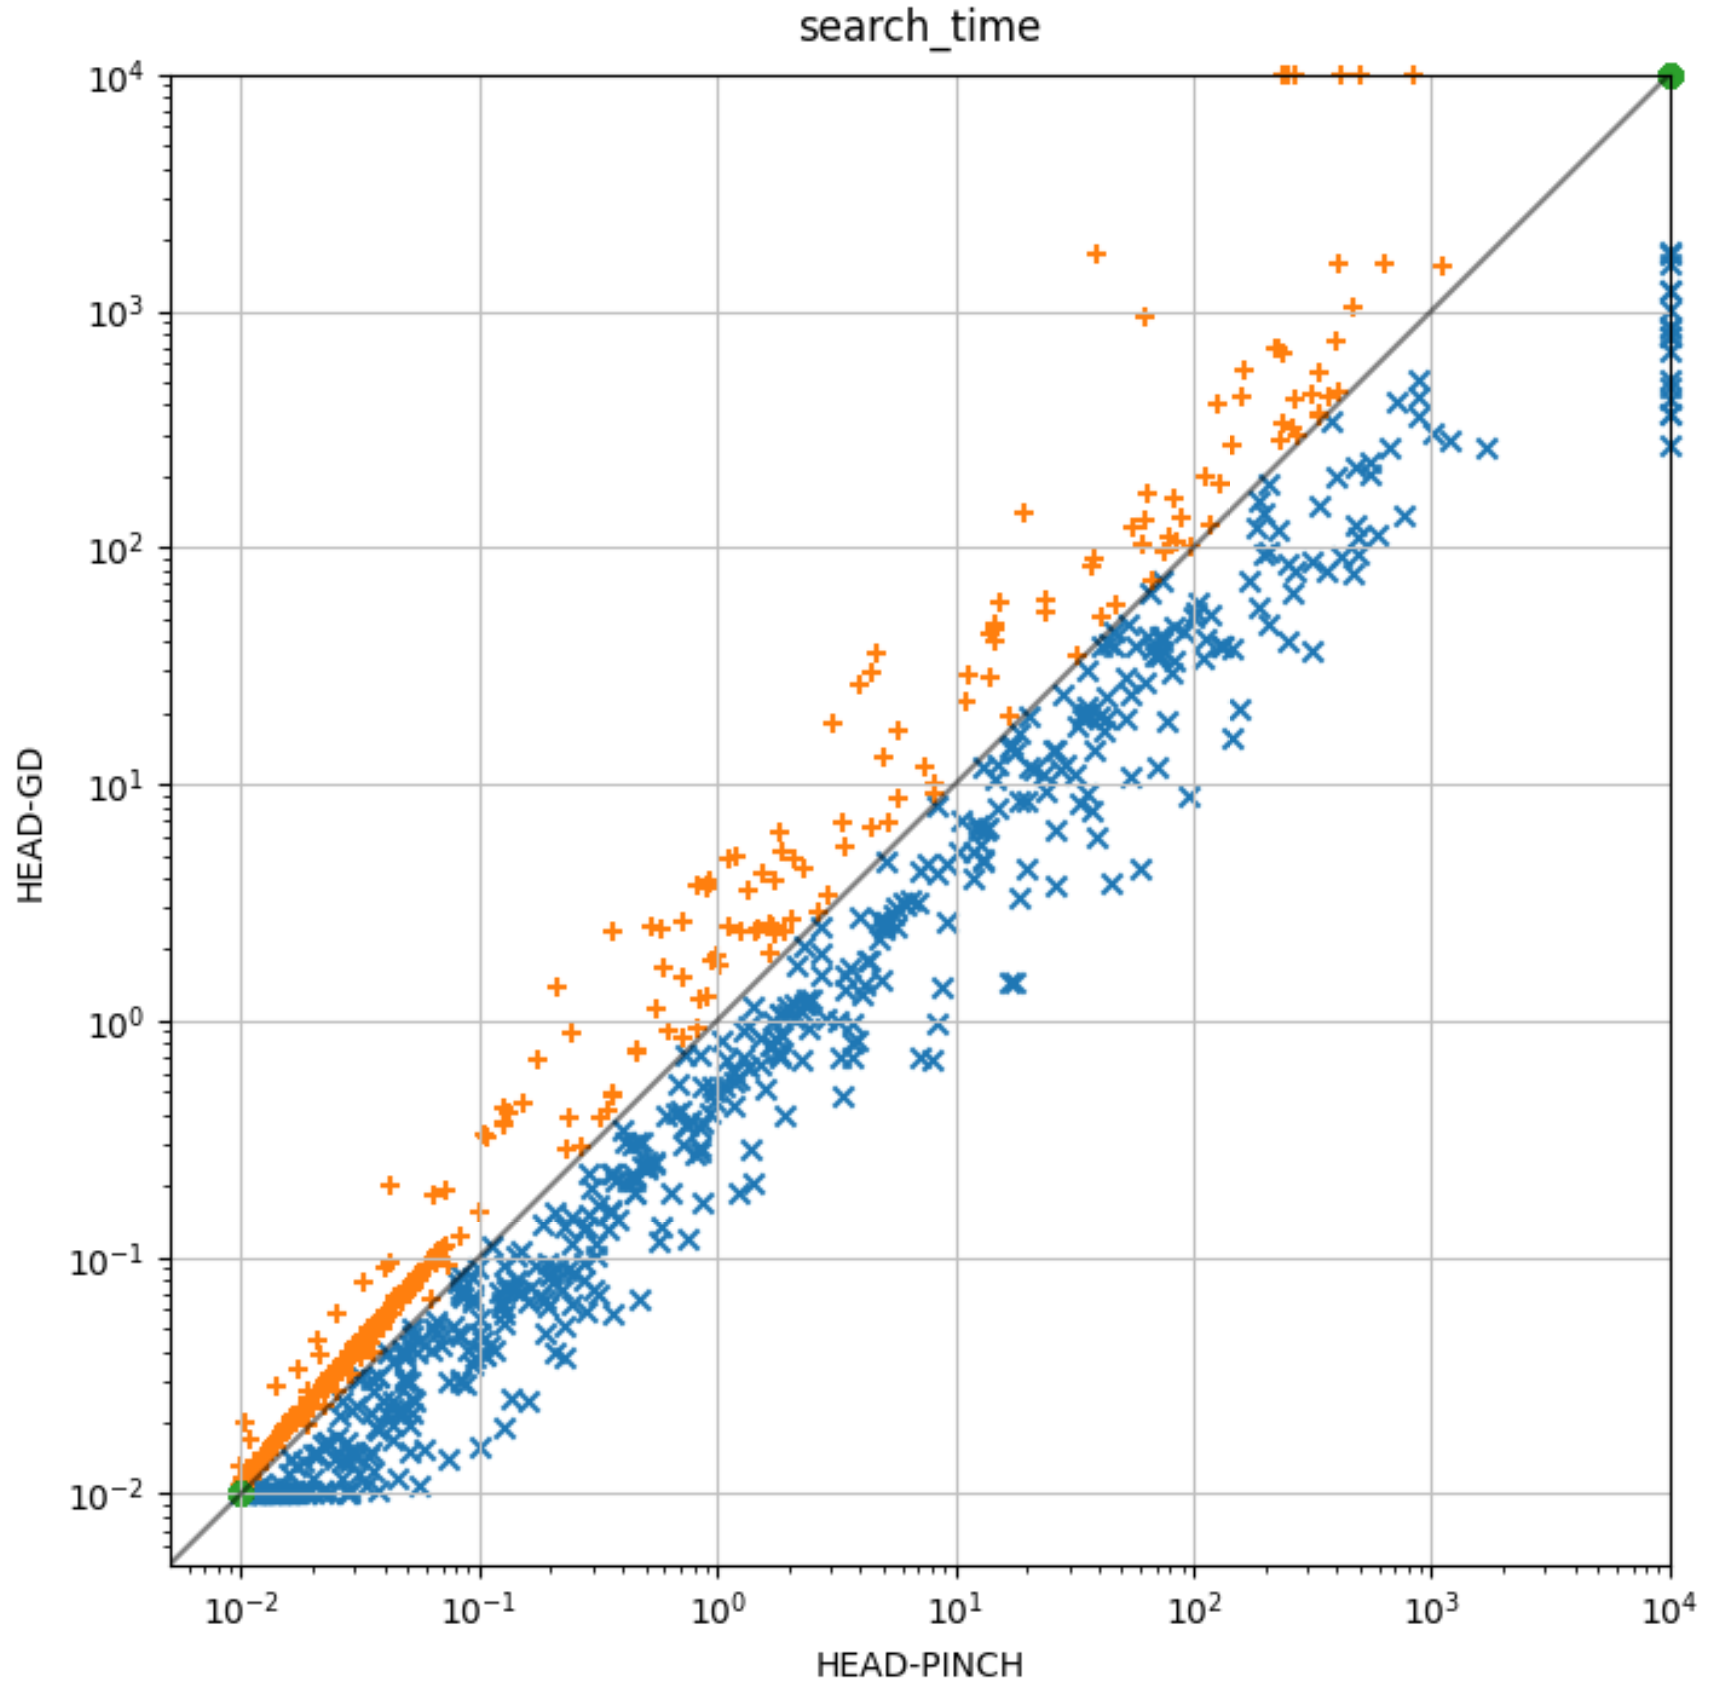
\includegraphics[width=\textwidth]{OP11.PNG}
  \end{minipage}
  \hfill
  \begin{minipage}[b]{0.40\textwidth}
    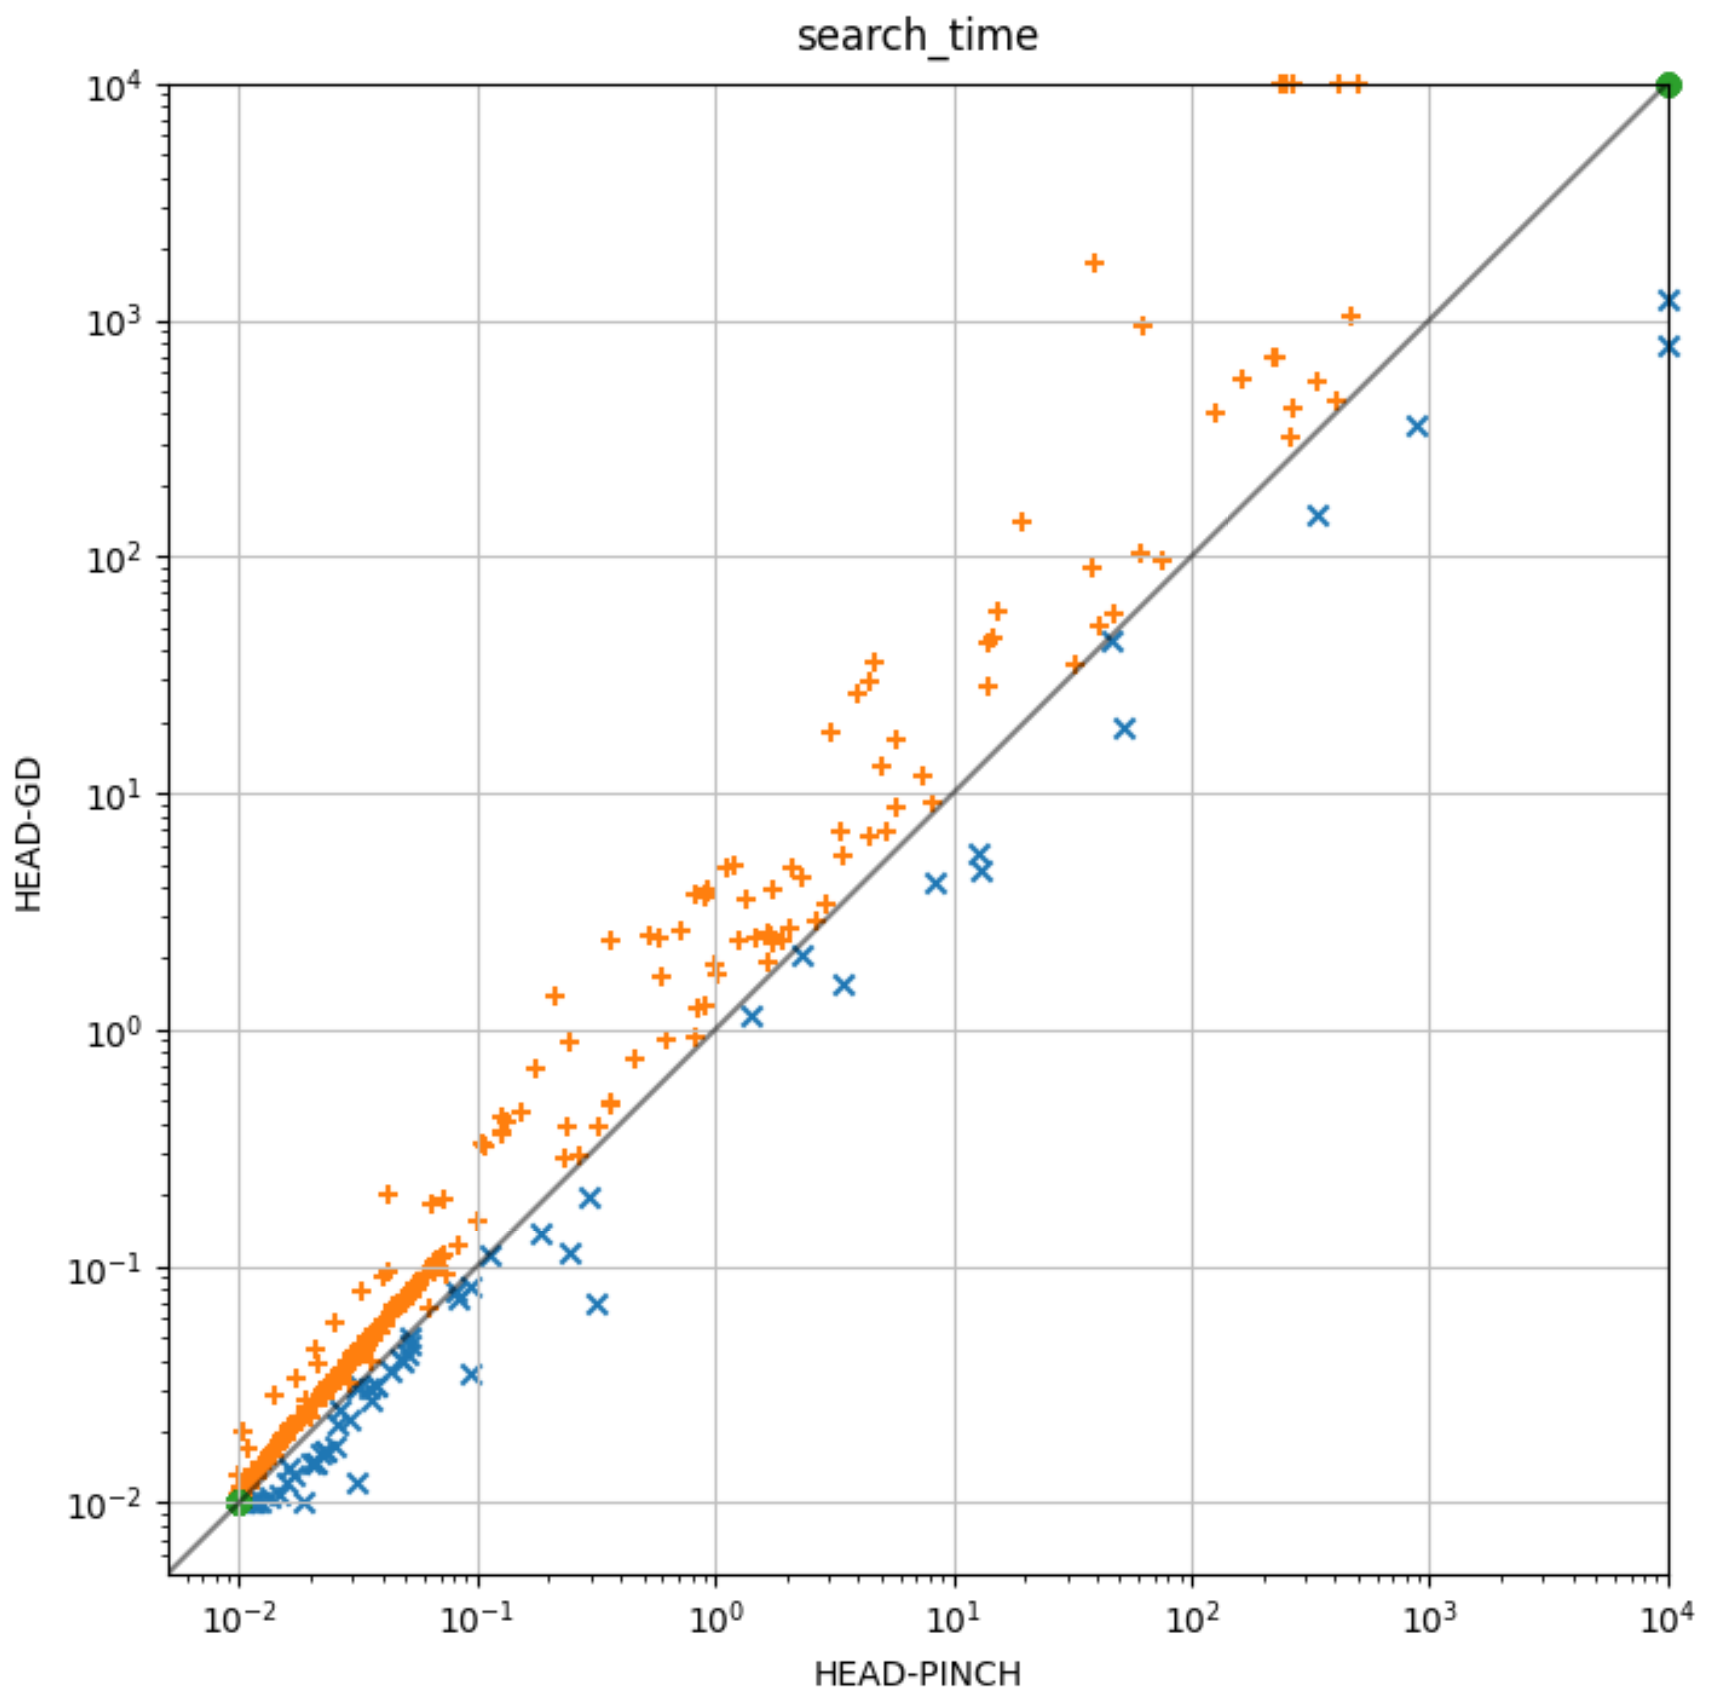
\includegraphics[width=\textwidth]{OP165.PNG}
    \caption{Search time plot with domains whose Factor 3 is less than 1.65 (left), less than 1.1(right). \textbf{Legend} Orange: PINCH favored, Blue: GD favored}
  \end{minipage}
\end{figure}\\
\begin{figure}[h]
  \centering
  \begin{minipage}[b]{0.40\textwidth}
    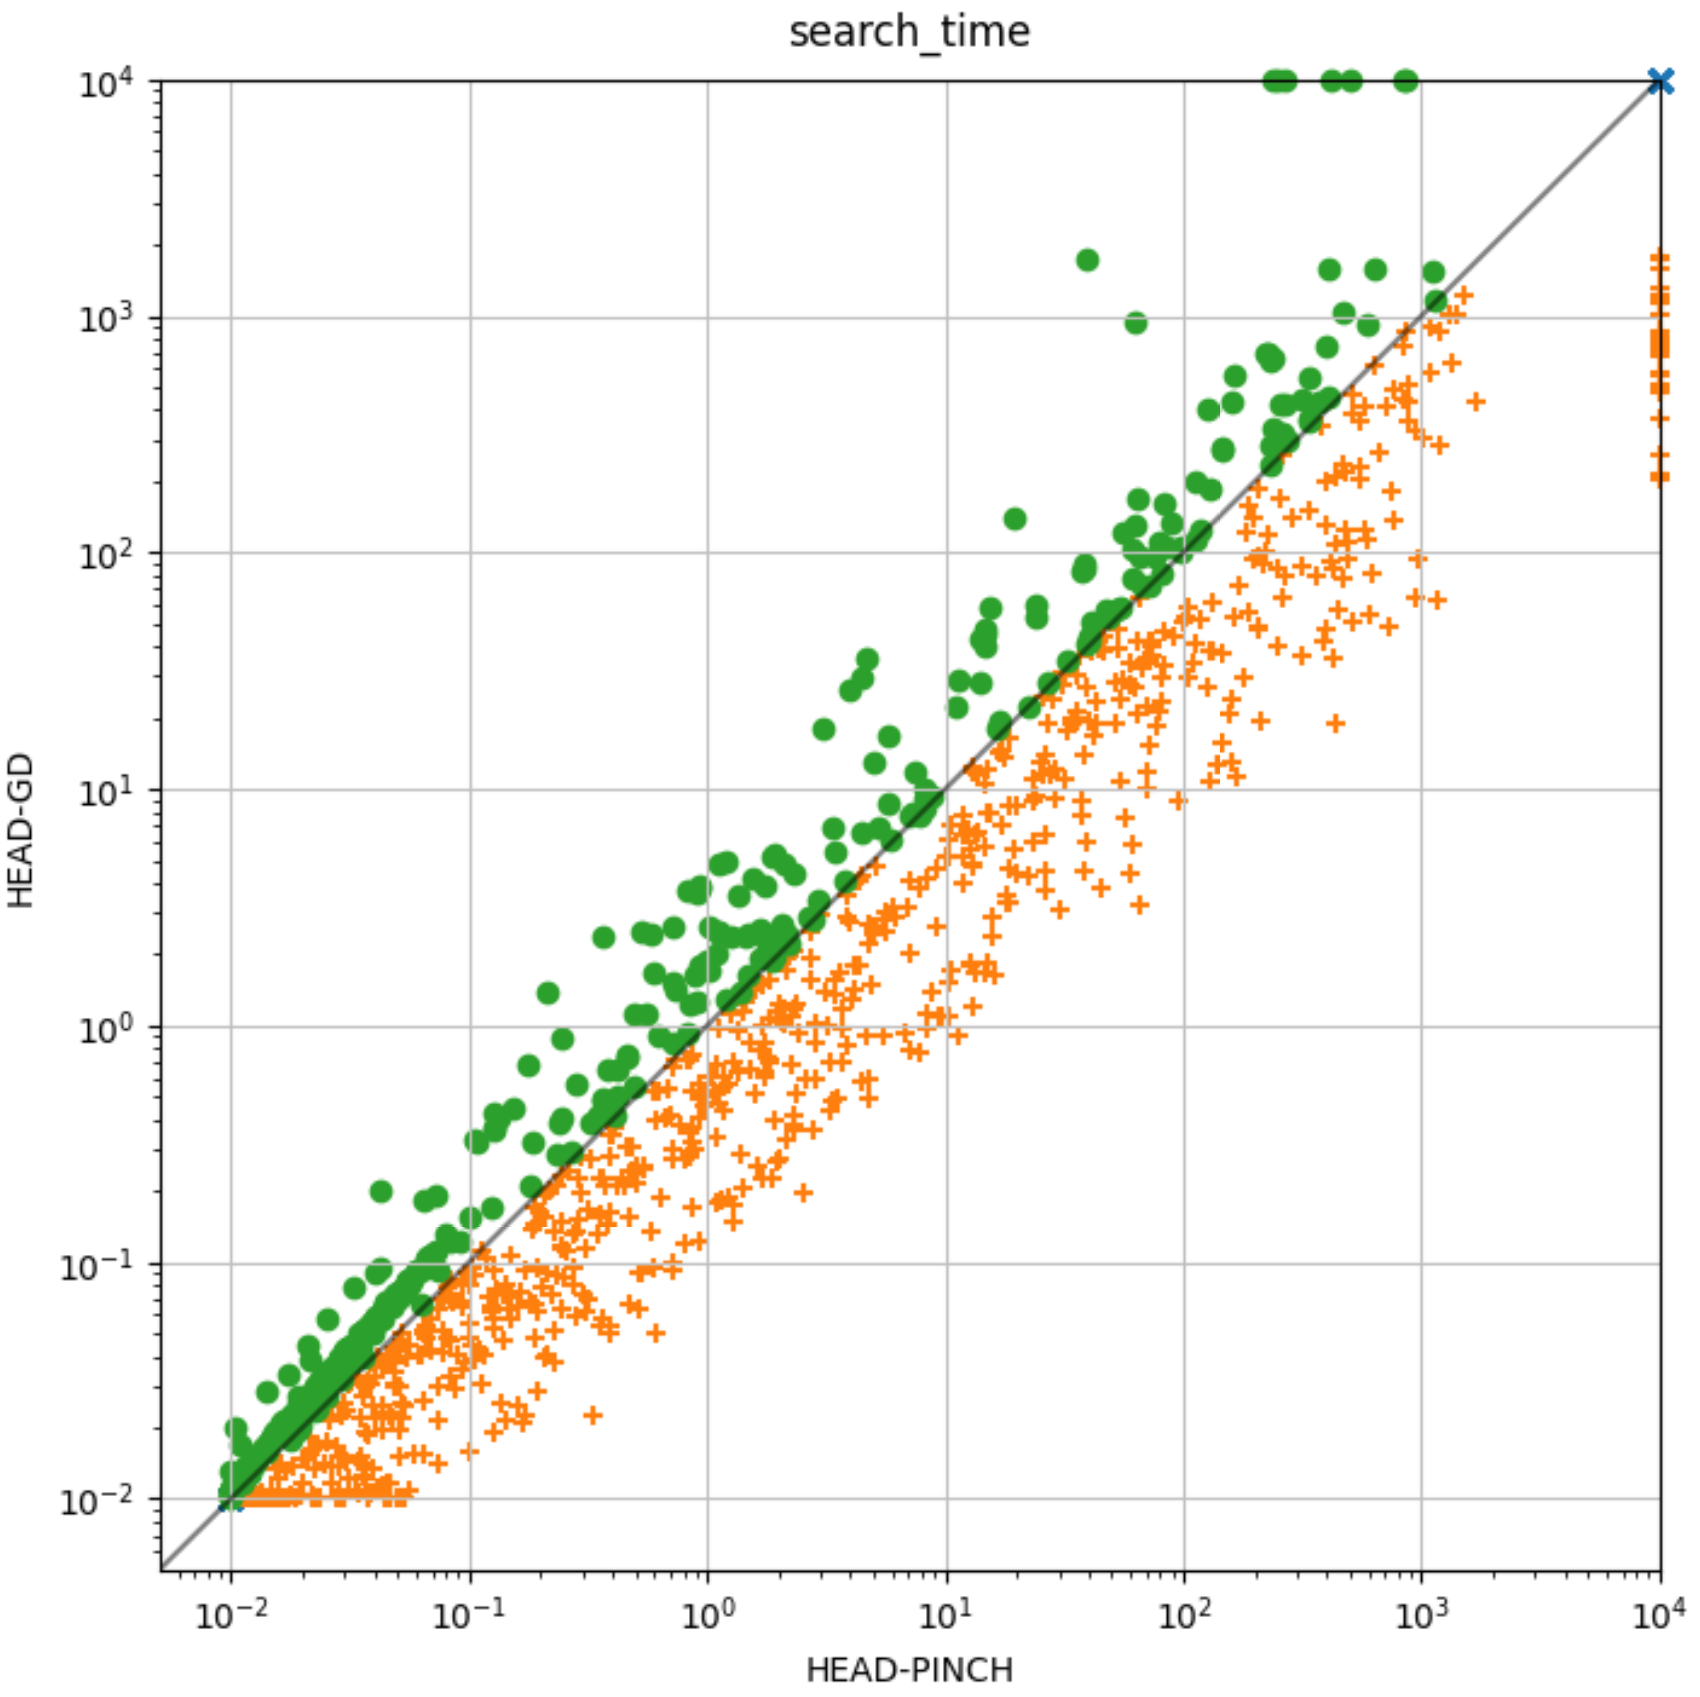
\includegraphics[width=\textwidth]{VAROP15.PNG}
  \end{minipage}
  \hfill
  \begin{minipage}[b]{0.40\textwidth}
    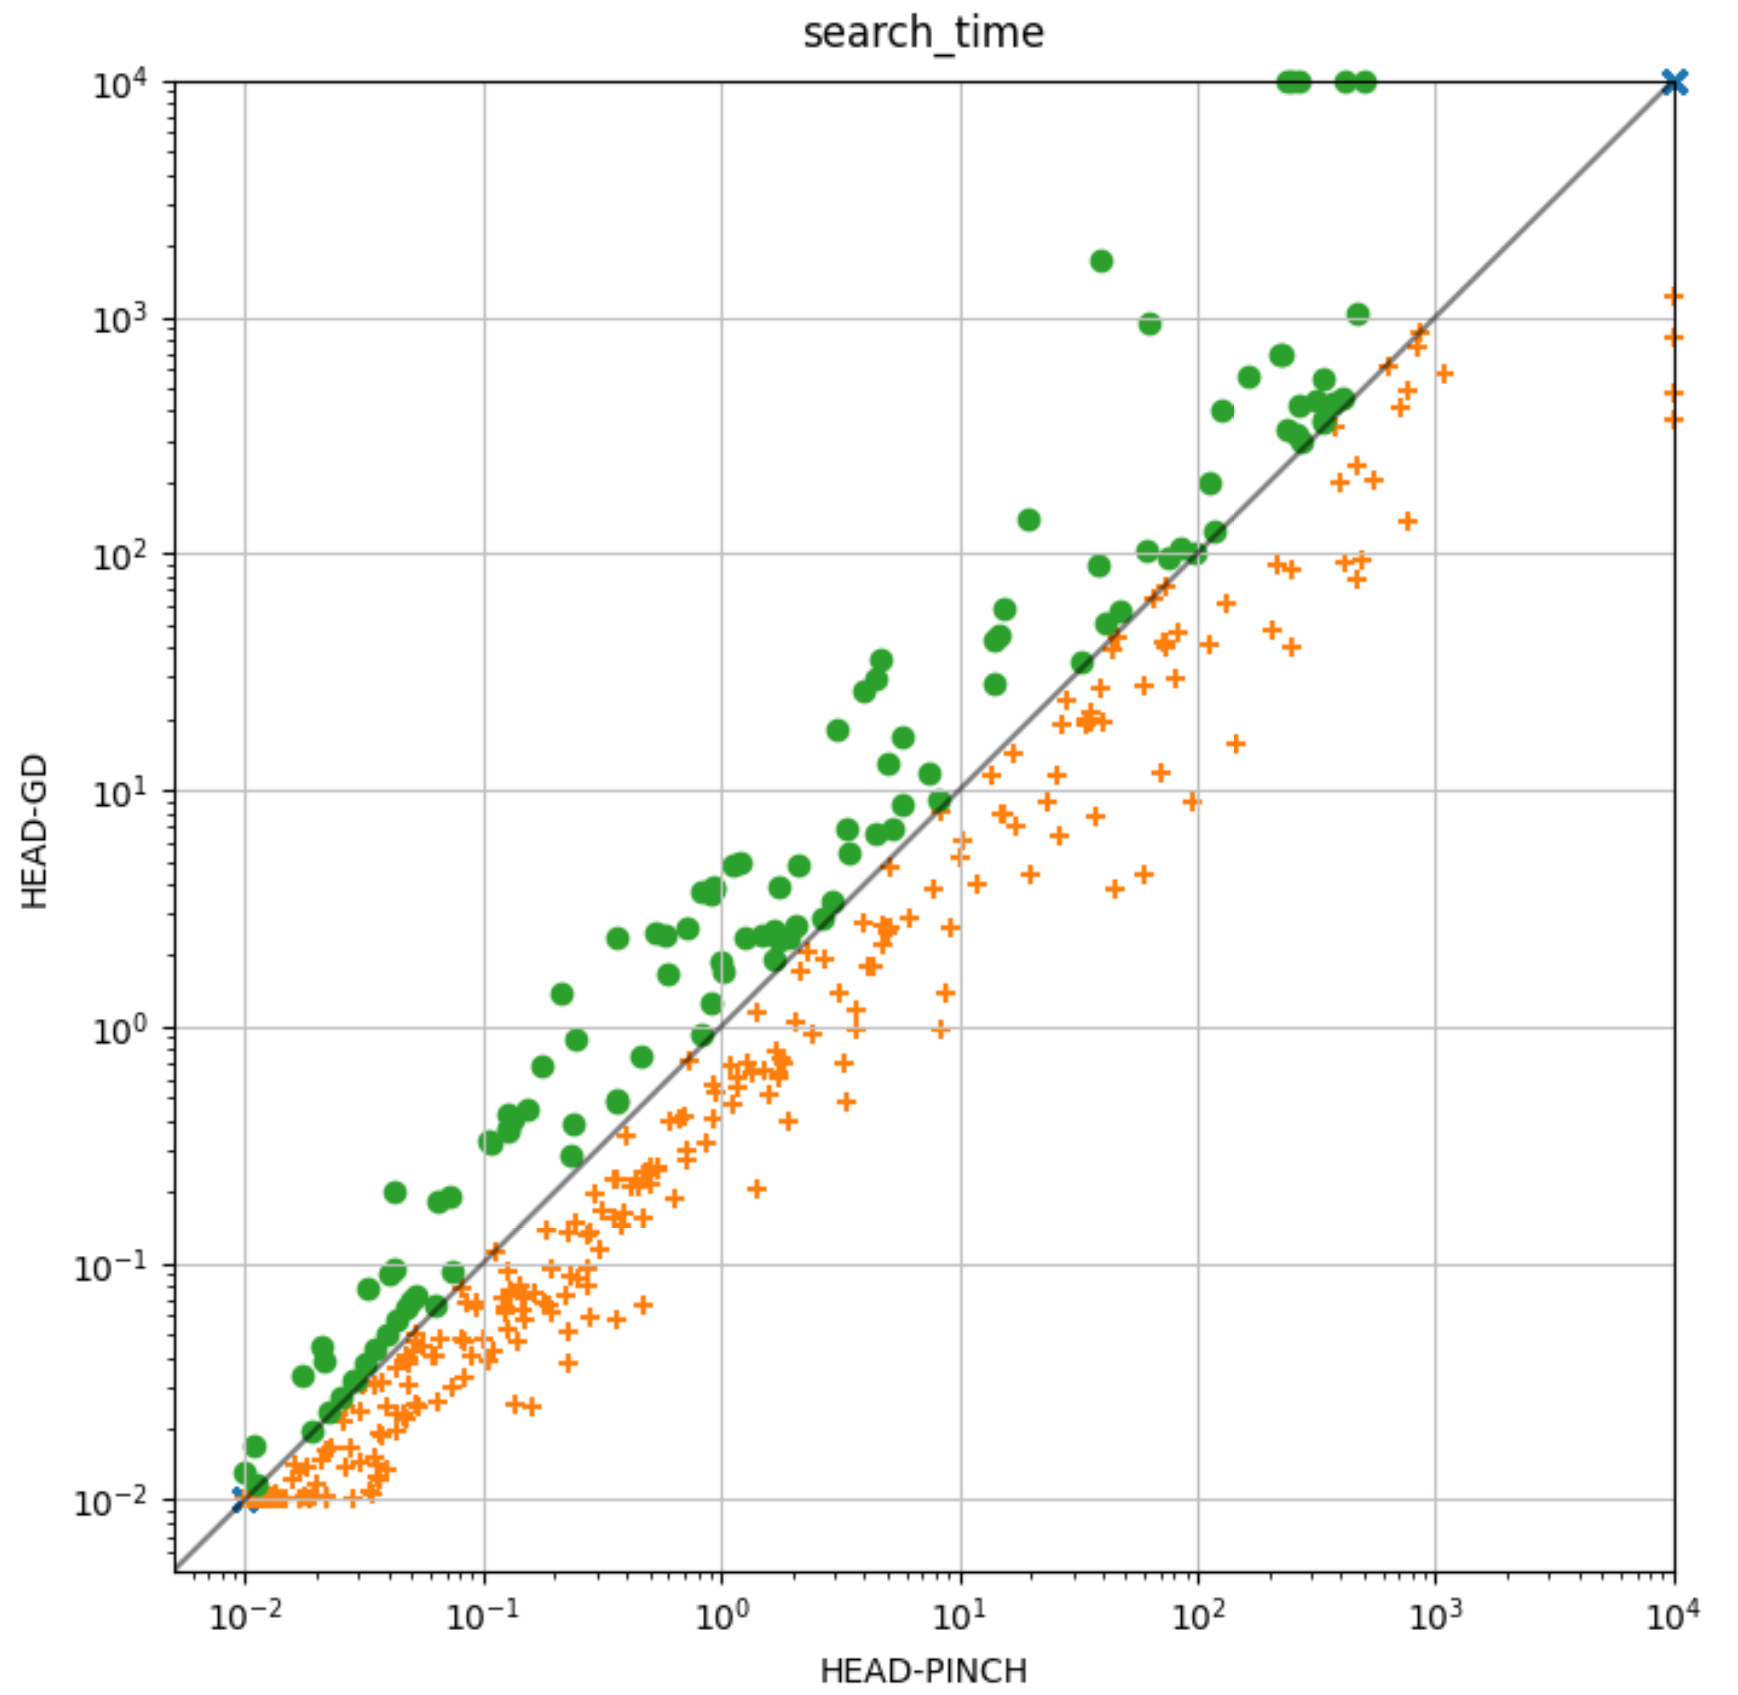
\includegraphics[width=\textwidth]{VAROP2.PNG}
    \caption{Search time plot with domains whose Factor 4 is more than 0.015 (left), more than 0.2 (right). \textbf{Legend} Green: PINCH favored, Orange: GD favored}
  \end{minipage}
\end{figure}
\newpage
As we continue to raise the standard for Factors 3 and/or 4 the performance of PINCH improves when compared to GD. There appears to be a strong correlation, in Figure 4.3 on the right picture PINCH beats GD by a factor of $\sim$3.3, the issue is that only a small number of domains contain the desired properties under which PINCH performs best. In Figure 4.5 we plot domains whose Factor 1/2 are \textit{better} and significantly \textit{better} than the mean.

\begin{figure}[h]
  \centering
  \begin{minipage}[b]{0.40\textwidth}
    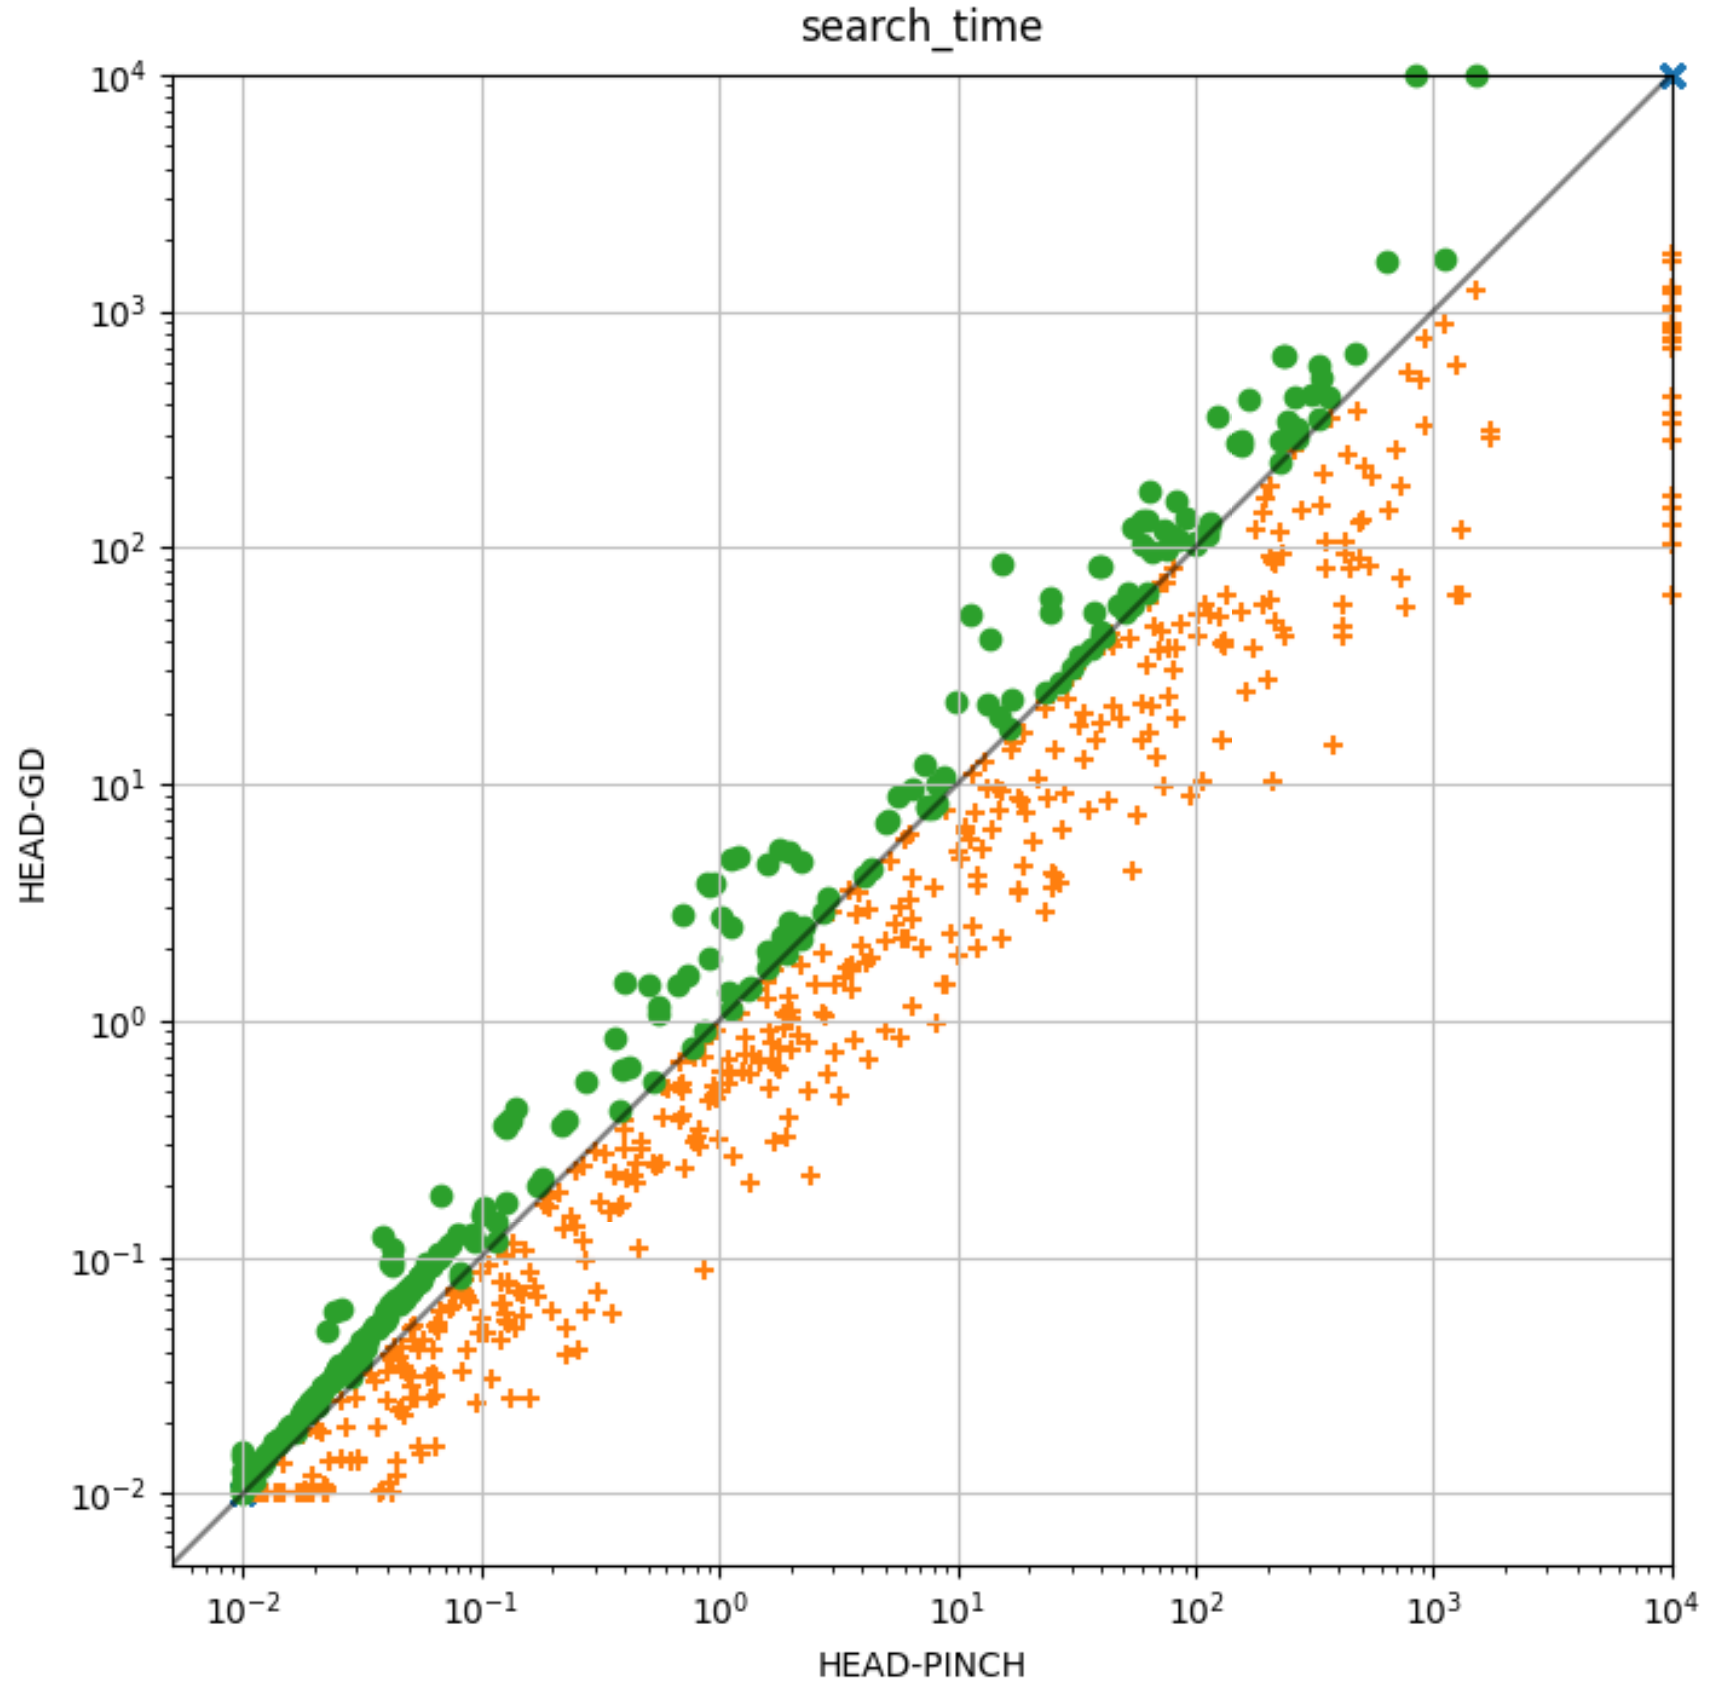
\includegraphics[width=\textwidth]{USETHIS.PNG}
  \end{minipage}
  \hfill
  \begin{minipage}[b]{0.40\textwidth}
    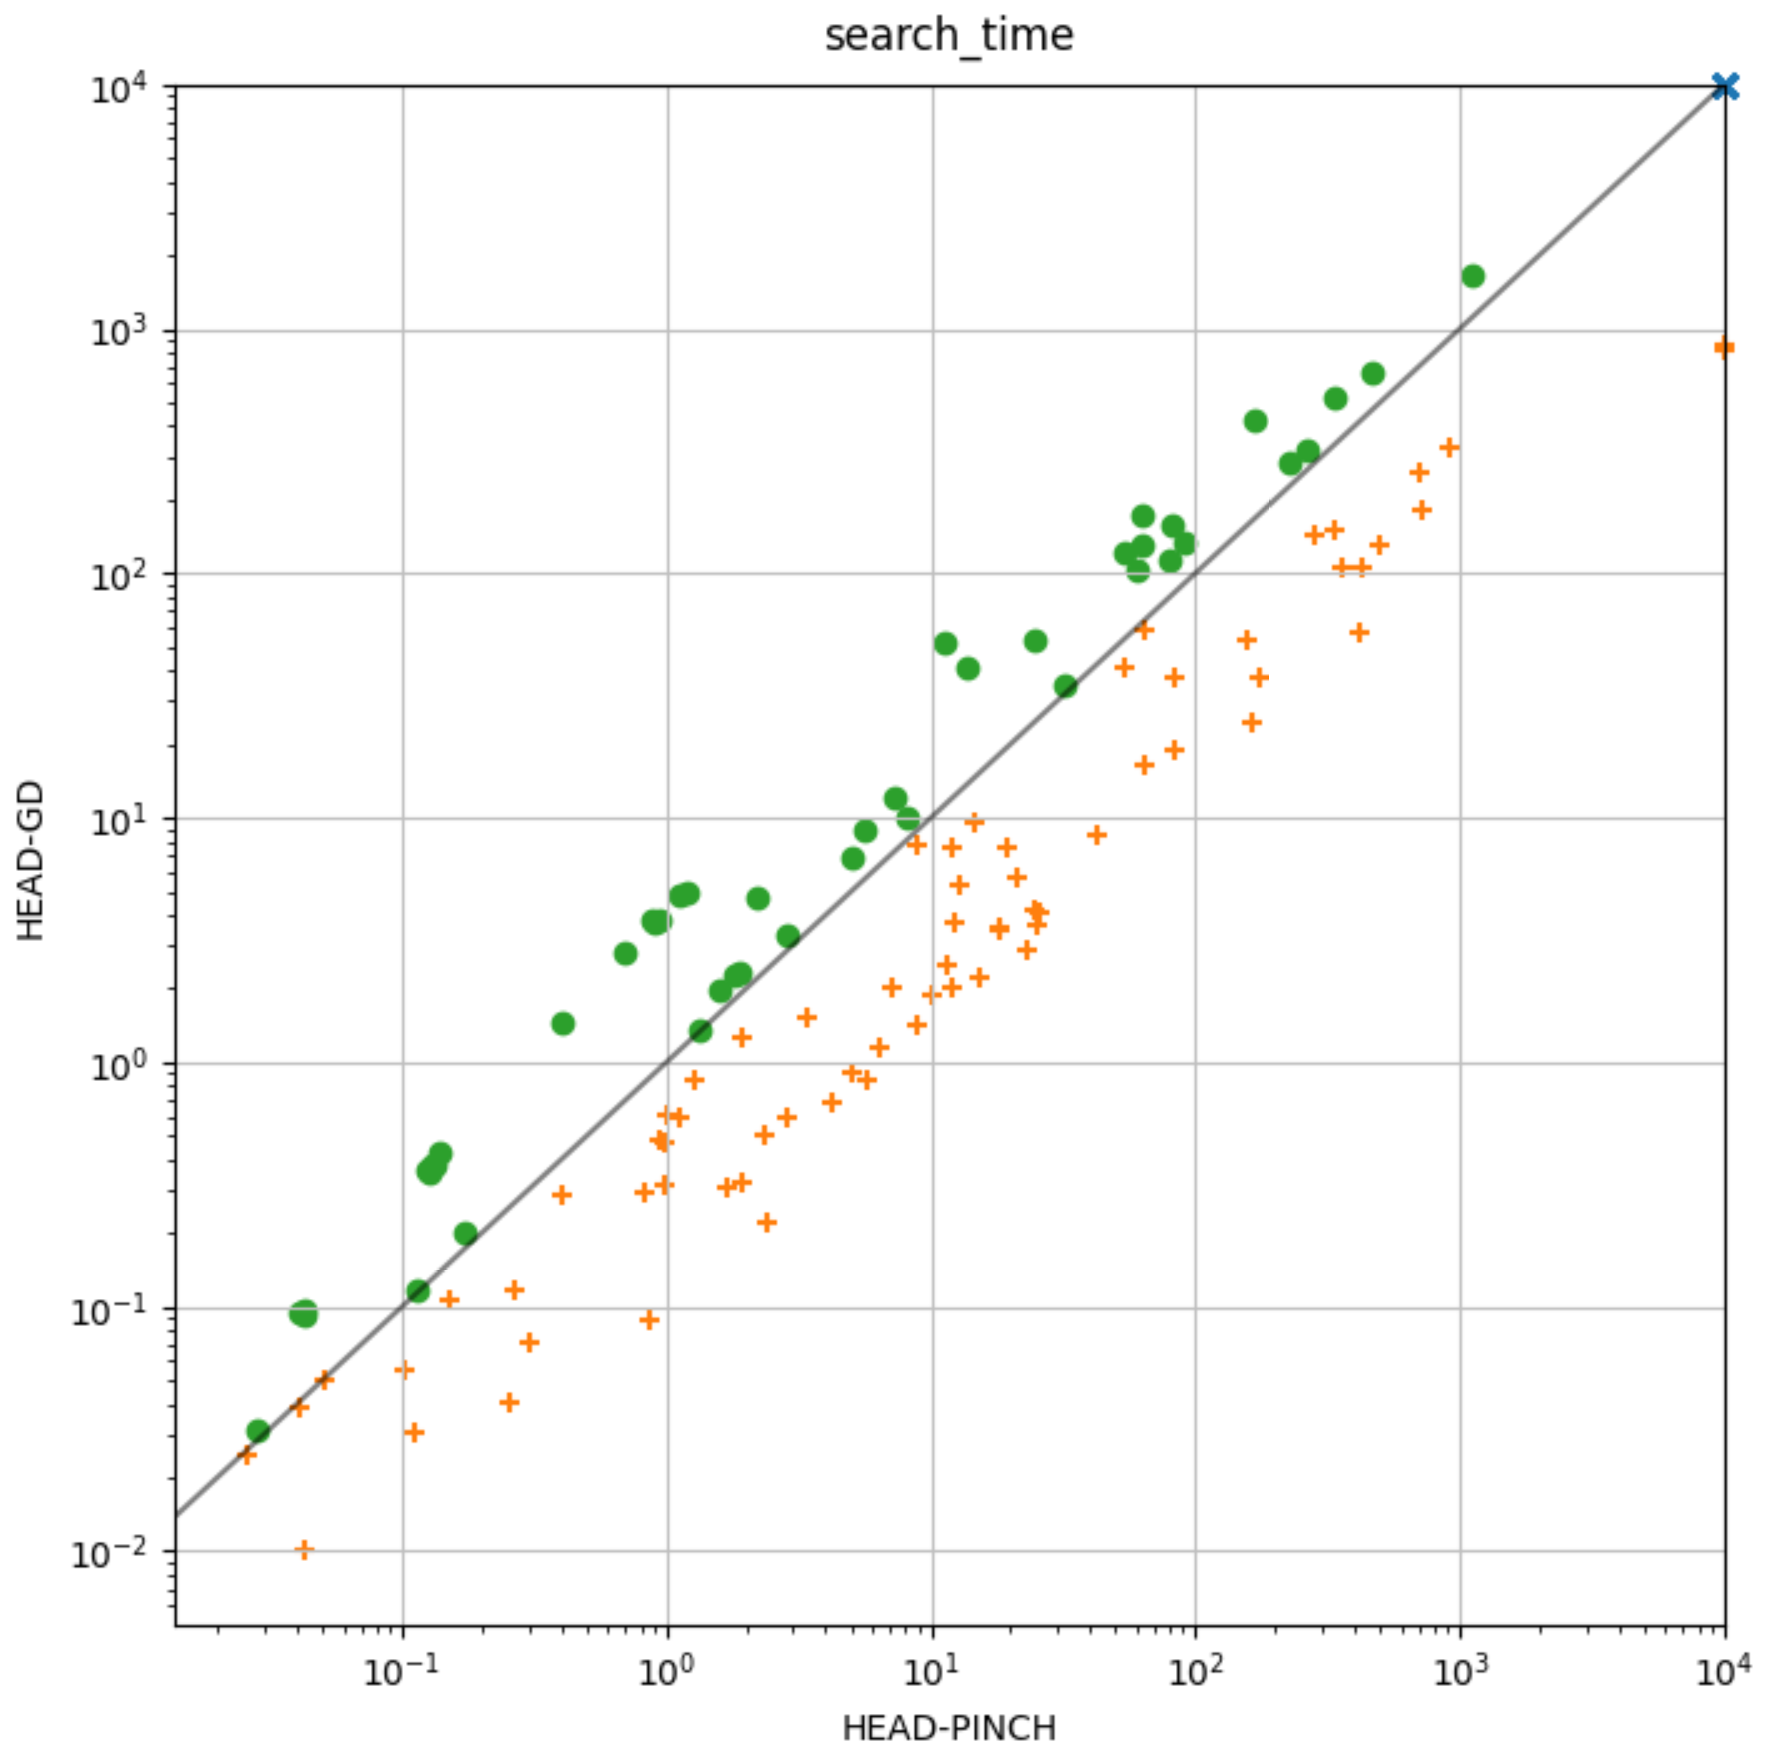
\includegraphics[width=\textwidth]{USETHIS2.PNG}
    \caption{Search time plot with domains whose Factor 1 and 2 is above 0.9/0.29 (left), above 0.98/0.4 (right). \textbf{Legend} Green: PINCH favored, Orange: GD favored}
  \end{minipage}
\end{figure}\\
As Table 4.4 suggested, insisting that all domains must be better than the mean in Factors 1 and 2 has not significantly improved the Performance of PINCH. If we raise the requirements to extreme amounts (Figure 4.5, right picture) we do get a slight improvement, with GD beating PINCH in roughly 2/3 of the covered domains, but we loose so many domains that it is hardly a good indicator.
\subsubsection{Conclusion}
Of the 4 factors that we have hypothesised would benefit the incremental aspect of PINCH and therefore PINCH as a whole, only 2 proved to have strong evidence in their favor. Perhaps the example, that was used in Chapter 4.2.3.1 from which Factor 1 and 2 were derived was too much unlike the types of state spaces that most instances induce. Factor 3 and 4 are clearly correlated with the performance of PINCH. We can conclude this since choosing domains that perform well in those factors drastically improves the performance of PINCH when compared to GD. What is especially interesting is that Factor 3 and 4 can be calculated prior to choosing a $h^a^d^d$ implementation, meaning that, if Factor 3 and 4 both appear to be \textit{good}, one could choose PINCH for the computation, and GD or a different $h^a^d^d$ implementation otherwise. Further research is needed to say when exactly PINCH reliably outperforms GD given Factor 3 and 4. In my runs PINCH started to \textit{beat} GD in more then 50\% of the covered domains roughly at around 1.2 for Factor 3 and 0.3 for Factor 4 but these numbers are based on a small sample-size. I have also not considered the positive effects of having both factors above a certain threshold, I only looked at each factor in isolation.
\newpage
\subsection{Comparing PINCH and GD Directly}
We can derive further factors if we compare PINCH and GD directly. 
\subsubsection{Introducing the Factors}
One thing we can compare is how many times PINCH has to adjusts the cost values of all $q \in V \cup A$. As mentioned before, PINCH updates the cost value of a given $q$ at most twice, while GD updates the cost value of all $q \in V \cup A$ exactly once. In the example from chapter 3.2, PINCH updates cost values 12 times. GD respectively would update cost values 13 times when applied to the same example. 
\begin{center}
\textit{\textbf{Factor 5:} The algorithm that adjusts fewer cost values has an advantage.}
\end{center}
Factor 5 does not take into consideration that PINCH and GD update cost values differently. PINCH updates exactly one cost value per $q \in V \cup A$ that is popped from the priority queue. GD only inserts $v \in V$ into the priority queue, it updates action cost values in the same iteration as it updates variable cost values. For the example from chapter 3.2, PINCH pops exactly 12 $q$ from the priority queue, GD only pops 7 $v$ from its priority queue when processing the same example.
\begin{center}
\textit{\textbf{Factor 6:} The algorithm that pops fewer $q \in V \cup A$ from its priority queue has an advantage.}
\end{center}
\subsubsection{Results}
To test for Factor 5 and 6 we simply count how many times on average for a state $s \in S$ PINCH and GD adjust their cost values or pop $q$ from their priority queues. \\
\begin{figure}
    \centering
    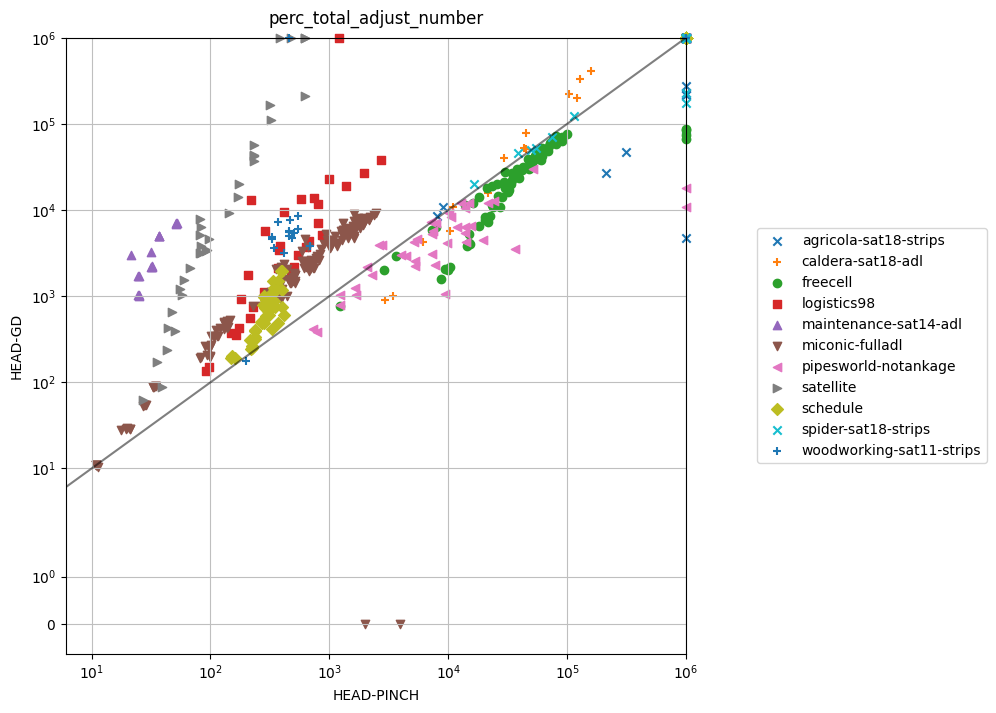
\includegraphics[width=.7\columnwidth]{plotSearchcost.png}
    \caption{total number of cost adjustments comparison plot between PINCH and GD}
    \label{fig:my_label}
\end{figure}
\newpage

Figure 4.6 shows us how many times PINCH adjusts its cost values on average compared to GD. PINCH updates its cost values at most twice, GD exactly once. In Figure 4.6 we can see that, thanks to the incremental benefit that PINCH has, PINCH tends to updated its cost values less than GD. Even for the GD favored domains the number of times cost values are adjusted are within a similar range.

\begin{figure}
    \centering
    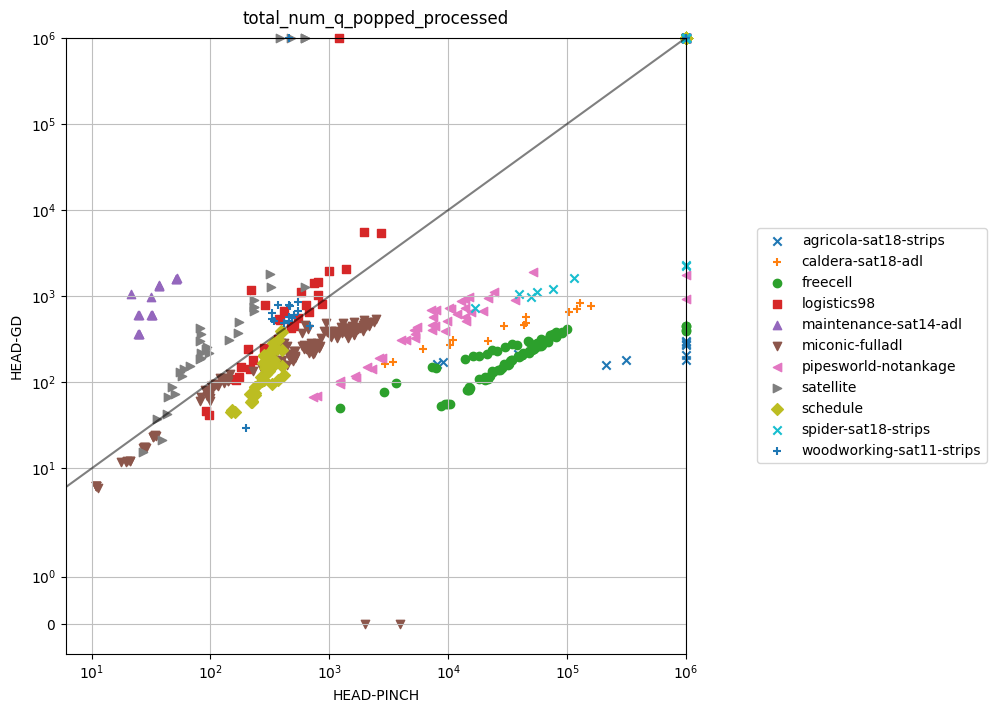
\includegraphics[width=.7\columnwidth]{plotSearch.png}
    \caption{total number of variables/actions popped out of the priority queue comparison plot between PINCH and GD}
    \label{fig:my_label}
\end{figure}
Figure 4.7 shows us how many times PINCH pops a variable or action out of its priority queue compared to GD. Since GD only stores variables in its priority queue it is expected that it pops fewer variables out of its priority queue. Even for domains that are PINCH favored GD tends to compare quite well. 
\subsubsection{Conclusion}
It is interesting, that Factor 5 appears to indicate that PINCH is the superior algorithm while Factor 6 does the opposite. While Factor 5 might be a good argument in favor of the benefits of PINCH, Factor 6 paints a different picture. Even though PINCH updates cost values less, it only achieves this by maintaining a fairly expensive priority queue. PINCH is required to store both variables and actions, in the worst case scenario it is required to insert and pop each of them twice. According to my testing maintenance of the priority queue is the single most time intensive part of PINCH, GD has an immense advantage here. The average number of $q$ popped form the priority queue for PINCH is 15519, for GD it is 432. Comparatively the average number of cost adjustments for PINCH is 15502, for GD it is 15701. Even tough PINCH does update cost values less, the way it achieves this comes at a huge price.
